% Task C18
% Source volume: lower
% Physical scan pages: 159--178
% Printed book pages: 147--166
% Transcribe only source content; omit running headers, footers, and printed page numbers.
\chapter{多元函数的极限与连续}

% BEGIN TRANSCRIPTION

本章讨论多元函数的极限与连续性。其中 §18.1 引进重极限与累次极限的概念，讨论了它们的相互关系，并介绍了一些常用方法。§18.2 讨论多元函数的连续性，介绍了一些多元函数连续的充分条件以及集合语言刻画连续性的命题，然后介绍紧集上的连续函数性质及其应用，最后对于向量值函数介绍了 $\RR^n$ 中的压缩映射原理。§18.3 是学习要点和两组参考题。

\section{多元函数的极限}

\subsection{重极限}

设点 $\vect{a}\in\RR^n$，$n$ 元函数 $f$ 在 $\vect{a}$ 的某个去心邻域中有定义，$A$ 为某一常数。若
\[
  \forall\varepsilon>0,\ \exists\delta>0,\quad
  0<\abs{\vect{x}-\vect{a}}<\delta
  \Longrightarrow \abs{f(\vect{x})-A}<\varepsilon,
\]
则称 $n$ 元函数 $f(\vect{x})$ 当 $\vect{x}\to\vect{a}$ 时以 $A$ 为极限（又称它是 $n$ 重极限），记为
\[
  \lim_{\vect{x}\to\vect{a}}f(\vect{x})=A
  \quad\text{或简记为}\quad
  f(\vect{x})\to A\quad(\vect{x}\to\vect{a}).
\]
用邻域的语言来描述，就是
\[
  \forall\varepsilon>0,\ \exists\delta>0,\quad
  \vect{x}\in O_\delta(\vect{a})\setminus\{\vect{a}\}
  \Longrightarrow f(\vect{x})\in O_\varepsilon(A).
\]

\begin{xremark}
在定义重极限时，可以放宽对函数定义域的要求，只要 $\vect{a}$ 是定义域的聚点即可。
\end{xremark}

从邻域的观点看，多元函数极限的定义与一元函数极限的定义完全一样。但现在是在高维空间中讨论，$\vect{x}\to\vect{a}$ 是指点 $\vect{x}$ 以任何方式或沿任何曲线趋于点 $\vect{a}$。其趋近方式要比一元函数的情形复杂得多。一个简单的例子是讨论
\[
  f(x,y)=\frac{xy}{x^2+y^2}
\]
在点 $(0,0)$ 的二重极限是否存在。容易看出，当点 $(x,y)$ 沿直线 $y=mx$（其中 $m$ 为任意实数）趋于点 $(0,0)$ 时，$f(x,y)$ 的极限为
\[
  \frac{m}{1+m^2},
\]
与 $m$ 有关。由此可以看出这个二元函数 $f(x,y)$ 在点 $(0,0)$ 的二重极限不存在。

与一元函数相仿，也可以定义自变量趋于 $\pm\infty$ 或 $\infty$ 时的极限，但现在是多个自变量，于是可以出现某一些自变量趋于一个定数，而另一些自变量趋于 $\pm\infty$ 或 $\infty$ 的情形。以两个自变量为例，可举出下述几种极限：
\begin{enumerate}[label=(\arabic*)]
  \item
  \[
  \begin{aligned}
    \lim_{(x,y)\to(\infty,\infty)}f(x,y)=A
    &\Longleftrightarrow \forall\varepsilon>0,\ \exists M>0,\\
    &\qquad \abs{x}>M,\ \abs{y}>M
    \Longrightarrow \abs{f(x,y)-A}<\varepsilon.
  \end{aligned}
  \]
  \item
  \[
  \begin{aligned}
    \lim_{(x,y)\to(x_0,+\infty)}f(x,y)=A
    &\Longleftrightarrow \forall\varepsilon>0,\ \exists\delta,M>0,\\
    &\qquad 0<\abs{x-x_0}<\delta,\ y>M
    \Longrightarrow \abs{f(x,y)-A}<\varepsilon.
  \end{aligned}
  \]
  \item
  \[
  \begin{aligned}
    \lim_{(x,y)\to(-\infty,y_0)}f(x,y)=A
    &\Longleftrightarrow \forall\varepsilon>0,\ \exists\delta,M>0,\\
    &\qquad x<-M,\ 0<\abs{y-y_0}<\delta
    \Longrightarrow \abs{f(x,y)-A}<\varepsilon.
  \end{aligned}
  \]
\end{enumerate}
还有其他一些情形，在此不一一列举。此外当 $A$ 为 $\pm\infty$ 或 $\infty$ 时，与一元函数类似，我们称之为广义极限或极限不存在（参见上册 98 页）。

多元函数的极限的惟一性、局部有界性、局部保号性、局部比较原理、四则运算法则、Cauchy 收敛准则以及 Heine 归结原理的叙述与论证完全与一元函数相仿，这里就不再重复了（参见上册第四章）。

求多元函数的极限有如下常用方法：
\begin{enumerate}[label=\arabic*.]
  \item 利用函数的连续性和函数极限的运算性质（多元函数的连续性将在下一节讨论）；
  \item 利用不等式缩放或使用夹逼定理；
  \item 利用变量替换化简或化为已知极限。对含有三角函数或幂指函数的二重极限可考虑它是否能通过变形或变量代换化为一元函数中的基本极限，如
  \[
    \lim_{t\to0}\frac{\sin t}{t}=1,\qquad
    \lim_{t\to0}\frac{\tan t}{t}=1,\qquad
    \lim_{t\to\infty}\left(1+\frac1t\right)^t=\ee
  \]
  等（参见上册 116 页题 9），然后利用这些基本极限去求重极限的值；
  \item 利用初等变形，如分母有理化、对指数形式取对数等等。
\end{enumerate}

\begin{xexample}[18.1.1]
求
\[
  \lim_{(x,y)\to(0,0)}\frac{x^3+y^3}{x^2+y^2}.
\]
\end{xexample}
\paragraph{分析}
直观上看分子的多项式次数高于分母的多项式次数，极限应该是 0。这种题目一般用极坐标变换后可化为一个有界量与无穷小量的乘积。
\begin{xsolution}
令 $x=r\cos\theta,y=r\sin\theta$，则
\[
  \lim_{(x,y)\to(0,0)}\frac{x^3+y^3}{x^2+y^2}
  =\lim_{r\to0}r(\cos^3\theta+\sin^3\theta)=0.
\]
\end{xsolution}

\begin{xexample}[18.1.2]
求
\[
  \lim_{(x,y)\to(0,0)}\frac{\sin(x^3+y^3)}{x^2+y^2}.
\]
\end{xexample}
\begin{xsolution}
由于
\[
  \abs{\sin(x^3+y^3)}\le \abs{x}^3+\abs{y}^3
  \le (\abs{x}+\abs{y})(x^2+y^2),
\]
从而
\[
  \lim_{(x,y)\to(0,0)}
  \abs*{\frac{\sin(x^3+y^3)}{x^2+y^2}}
  \le
  \lim_{(x,y)\to(0,0)}(\abs{x}+\abs{y})=0.
\]
所以
\[
  \lim_{(x,y)\to(0,0)}\frac{\sin(x^3+y^3)}{x^2+y^2}=0.
\]
\end{xsolution}
\begin{xremark}
也可对 $\sin(x^3+y^3)$ 用一元 Taylor 展式
\[
  \sin(x^3+y^3)=x^3+y^3+\littleo(\abs{x}^3+\abs{y}^3)
  \qquad(\abs{x}+\abs{y}\to0).
\]
\end{xremark}

\begin{xexample}[18.1.3]
求 $\displaystyle\lim_{(x,y)\to(0,0)}f(x,y)$，其中
\[
  f(x,y)=
  \begin{cases}
    \dfrac{\sin xy}{x}, & x\ne0,\\[4pt]
    y, & x=0,\ y\ne0.
  \end{cases}
\]
\end{xexample}
\begin{xsolution}
由于
\[
  \abs{f(x,y)}=
  \begin{cases}
    \abs*{\dfrac{\sin xy}{x}}\le\abs{y}, & x\ne0,\\[4pt]
    \abs{y}, & x=0,\ y\ne0,
  \end{cases}
\]
所以
\[
  \lim_{(x,y)\to(0,0)}\abs{f(x,y)}
  \le \lim_{(x,y)\to(0,0)}\abs{y}=0.
\]
于是
\[
  \lim_{(x,y)\to(0,0)}f(x,y)=0.
\]
\end{xsolution}

\begin{xexample}[18.1.4]
求极限
\[
  \lim_{(x,y)\to(0,0)}(x^2+y^2)^{xy}.
\]
\end{xexample}
\begin{xsolution}
先求其对数的极限
\[
  \lim_{(x,y)\to(0,0)}xy\ln(x^2+y^2).
\]
设 $r=\sqrt{x^2+y^2}$，由于
\[
  \abs{xy\ln(x^2+y^2)}\le r^2\abs{\ln r^2}\to0
  \qquad(r\to0^+),
\]
所以
\[
  \lim_{(x,y)\to(0,0)}xy\ln(x^2+y^2)=0,
\]
故
\[
  \lim_{(x,y)\to(0,0)}(x^2+y^2)^{xy}=1.
\]
\end{xsolution}

\begin{xexample}[18.1.5]
证明：
\[
  \lim_{(x,y)\to(+\infty,+\infty)}
  \left(\frac{xy}{x^2+y^2}\right)^{x^2}=0.
\]
\end{xexample}
\begin{xproof}
此题底数的极限并不存在，但可用夹逼方法。注意到 $x>0,y>0$ 时
\[
  0<\frac{xy}{x^2+y^2}\le\frac12,
\]
所以
\[
  0<\left(\frac{xy}{x^2+y^2}\right)^{x^2}
  \le\left(\frac12\right)^{x^2}.
\]
由于
\[
  \lim_{(x,y)\to(+\infty,+\infty)}\left(\frac12\right)^{x^2}=0,
\]
从而有
\[
  \lim_{(x,y)\to(+\infty,+\infty)}
  \left(\frac{xy}{x^2+y^2}\right)^{x^2}=0.
\]
\end{xproof}

关于证明重极限不存在的方法，我们将在累次极限之后介绍。

\subsection{累次极限}

为方便起见，在 $\RR^2$ 中讨论，设 $f(x,y)$ 在点 $(x_0,y_0)$ 的某个去心邻域上有定义，称下列两个极限（如果存在的话）
\[
  \lim_{y\to y_0}\lim_{x\to x_0}f(x,y),
  \qquad
  \lim_{x\to x_0}\lim_{y\to y_0}f(x,y)
\]
分别是函数 $f$ 在点 $(x_0,y_0)$ 的先 $x$ 后 $y$ 的二次极限和先 $y$ 后 $x$ 的二次极限，统称它们是累次极限。

重极限与累次极限的关系反映在下面的命题中。

\begin{xproposition}[18.1.1]
当重极限存在且
\[
  \lim_{(x,y)\to(x_0,y_0)}f(x,y)=A
\]
时，
\begin{enumerate}[label=(\arabic*)]
  \item 如果 $y\ne y_0$ 时，$\displaystyle\lim_{x\to x_0}f(x,y)$ 存在，则
  \[
    \lim_{y\to y_0}\lim_{x\to x_0}f(x,y)=A;
  \]
  \item 如果 $x\ne x_0$ 时，$\displaystyle\lim_{y\to y_0}f(x,y)$ 存在，则
  \[
    \lim_{x\to x_0}\lim_{y\to y_0}f(x,y)=A.
  \]
\end{enumerate}
\end{xproposition}

由此命题可见：当重极限和某个累次极限都存在时，则该累次极限的值应该等于重极限的值。但在一般情况下，重极限与累次极限没有什么必然的关系。

当重极限存在时，两个二次极限可以都不存在，也可以一个存在而另一个不存在，例如
\[
  f(x,y)=
  \begin{cases}
    x\sin\dfrac1y, & y\ne0,\\[4pt]
    0, & y=0.
  \end{cases}
\]
此时
\[
  \lim_{(x,y)\to(0,0)}f(x,y)
  =\lim_{y\to0}\lim_{x\to0}f(x,y)=0,
\]
但
\[
  \lim_{x\to0}\lim_{y\to0}f(x,y)
\]
不存在。

当重极限不存在时，可以是两个二次极限存在且相等，也可以是两个二次极限存在但不相等，还可以是两个二次极限中一个存在而另一个不存在。例如
\[
  f(x,y)=\frac{y}{x},\qquad x\ne0,
\]
显然有
\[
  \lim_{x\to0}\lim_{y\to0}f(x,y)=0,
\]
但是
\[
  \lim_{(x,y)\to(0,0)}f(x,y)
  \quad\text{与}\quad
  \lim_{y\to0}\lim_{x\to0}f(x,y)
\]
都不存在。

\subsection{证明函数的重极限不存在的常用方法}

\begin{enumerate}[label=\arabic*.]
  \item 找两种特殊的趋近方式，使得在两种方式下函数的极限值不同。例如
  \[
    f(x,y)=
    \begin{cases}
      0, & x^2\le\abs{y}\ \text{或}\ y=0,\\
      1, & \text{其他}.
    \end{cases}
  \]
  当点 $(x,y)$ 沿过原点的任何直线 $y=kx$ 趋于点 $(0,0)$ 时，有
  \[
    \lim_{(x,y=kx)\to(0,0)}f(x,y)=0.
  \]
  但点 $(x,y)$ 沿曲线 $y=\dfrac12x^2$ 趋于点 $(0,0)$ 时
  \[
    \lim_{(x,y=x^2/2)\to(0,0)}f(x,y)=1,
  \]
  所以 $f(x,y)$ 在点 $(0,0)$ 处的重极限不存在。

  \item 证明两个累次极限存在但不相等，例如
  \[
    f(x,y)=\frac{x^2-y^2}{x^2+y^2}.
  \]
  由于
  \[
    \lim_{x\to0}\lim_{y\to0}f(x,y)=1,
    \qquad
    \lim_{y\to0}\lim_{x\to0}f(x,y)=-1,
  \]
  可见重极限不存在：因为如果重极限存在，两个累次极限又存在，由命题 18.1.1 知这三个极限值应该相等。
\end{enumerate}

\subsection{思考题}

\begin{xthought}[1]
证明多元函数极限的 Heine 归结原理：设点 $\vect{a}\in\RR^n,A\in\RR$，则 $\displaystyle\lim_{\vect{x}\to\vect{a}}f(\vect{x})=A$ 的充分必要条件是：对满足条件 $\vect{x}_n\ne\vect{a}$（$n=1,2,\ldots$）、$\displaystyle\lim_{n\to\infty}\vect{x}_n=\vect{a}$ 的每个点列 $\{\vect{x}_n\}$，都有
  \[
    \lim_{n\to\infty}f(\vect{x}_n)=A.
  \]
  （参见上册 104--105 页。）
\end{xthought}
\begin{xsolution}
先证必要性。设
\[
  \lim_{\vect{x}\to\vect{a}}f(\vect{x})=A,
\]
并取任意满足 $\vect{x}_n\ne\vect{a}$、$\vect{x}_n\to\vect{a}$ 的点列。给定 $\varepsilon>0$，由极限定义，存在 $\delta>0$，使得
\[
  0<\abs{\vect{x}-\vect{a}}<\delta
  \Longrightarrow
  \abs{f(\vect{x})-A}<\varepsilon.
\]
由于 $\vect{x}_n\to\vect{a}$，存在 $N$，当 $n\ge N$ 时
\[
  0<\abs{\vect{x}_n-\vect{a}}<\delta,
\]
于是
\[
  \abs{f(\vect{x}_n)-A}<\varepsilon.
\]
故 $f(\vect{x}_n)\to A$。

再证充分性。反设 $\lim_{\vect{x}\to\vect{a}}f(\vect{x})\ne A$。则存在 $\varepsilon_0>0$，使得对任意 $\delta>0$，总能找到定义域中的点 $\vect{x}$ 满足
\[
  0<\abs{\vect{x}-\vect{a}}<\delta,
  \qquad
  \abs{f(\vect{x})-A}\ge\varepsilon_0.
\]
令 $\delta=1/n$，依次选取 $\vect{x}_n$，使
\[
  0<\abs{\vect{x}_n-\vect{a}}<\frac1n,
  \qquad
  \abs{f(\vect{x}_n)-A}\ge\varepsilon_0.
\]
于是 $\vect{x}_n\to\vect{a}$，但 $f(\vect{x}_n)$ 不趋于 $A$，与题设矛盾。因此
\[
  \lim_{\vect{x}\to\vect{a}}f(\vect{x})=A.
\]
\end{xsolution}


\begin{xthought}[2]
证明多元函数极限的 Cauchy 收敛准则：函数 $f(\vect{x})$ 在点 $\vect{a}$ 有极限的充分必要条件是对每一个 $\varepsilon>0$，$\exists\delta>0$，使得对于 $O_\delta(\vect{a})\setminus\{\vect{a}\}$ 中的每一对点 $\vect{x}',\vect{x}''$，满足不等式
  \[
    \abs{f(\vect{x}')-f(\vect{x}'')}<\varepsilon.
  \]
\end{xthought}
\begin{xsolution}
必要性。设
\[
  \lim_{\vect{x}\to\vect{a}}f(\vect{x})=A.
\]
给定 $\varepsilon>0$，取 $\delta>0$，使
\[
  0<\abs{\vect{x}-\vect{a}}<\delta
  \Longrightarrow
  \abs{f(\vect{x})-A}<\frac\varepsilon2.
\]
于是对任意 $\vect{x}',\vect{x}''\in O_\delta(\vect{a})\setminus\{\vect{a}\}$，
\[
  \abs{f(\vect{x}')-f(\vect{x}'')}
  \le
  \abs{f(\vect{x}')-A}+\abs{f(\vect{x}'')-A}
  <\varepsilon.
\]

充分性。设题中 Cauchy 条件成立。由于 $\vect{a}$ 是定义域的聚点，可取定义域中的点列 $\vect{x}_n\ne\vect{a}$，使 $\vect{x}_n\to\vect{a}$。给定 $\varepsilon>0$，取 Cauchy 条件中的 $\delta>0$。当 $m,n$ 足够大时，
\[
  \vect{x}_m,\vect{x}_n\in O_\delta(\vect{a})\setminus\{\vect{a}\},
\]
所以
\[
  \abs{f(\vect{x}_m)-f(\vect{x}_n)}<\varepsilon.
\]
故 $\{f(\vect{x}_n)\}$ 是实数 Cauchy 列，从而收敛，记
\[
  f(\vect{x}_n)\to A.
\]

任取另一列 $\vect{y}_n\ne\vect{a}$、$\vect{y}_n\to\vect{a}$，把两列交错组成
\[
  \vect{z}_{2n}=\vect{x}_n,
  \qquad
  \vect{z}_{2n-1}=\vect{y}_n.
\]
仍有 $\vect{z}_n\to\vect{a}$，由同一 Cauchy 条件知 $\{f(\vect{z}_n)\}$ 是 Cauchy 列，故收敛。其偶数项子列已经趋于 $A$，所以整列极限只能是 $A$，于是奇数项子列也满足
\[
  f(\vect{y}_n)\to A.
\]
由上一题的 Heine 归结原理，得到
\[
  \lim_{\vect{x}\to\vect{a}}f(\vect{x})=A.
\]
\end{xsolution}


\subsection{关于累次极限换序}

命题 18.1.1 告诉我们，如果在某一点二元函数的重极限与两个累次极限都存在，则对 $x$ 和 $y$ 取极限的顺序可以交换，即
\[
  \lim_{x\to x_0}\lim_{y\to y_0}f(x,y)
  =\lim_{y\to y_0}\lim_{x\to x_0}f(x,y).
\]
如果我们并不知道重极限是否存在或者甚至知道重极限不存在，那么在什么条件下，累次极限可以交换次序呢？下面的命题回答了这个问题。

\begin{xproposition}[18.1.2]
$f(x,y)$ 在点 $(x_0,y_0)$ 的一个去心邻域上有定义，如果
\begin{enumerate}[label=(\arabic*)]
  \item 对 $x_0$ 临近的每个 $x\ne x_0$，$\displaystyle\lim_{y\to y_0}f(x,y)=g(x)$ 存在；
  \item $\displaystyle\lim_{x\to x_0}f(x,y)=h(y)$ 关于 $y$ 在 $0<\abs{y-y_0}<\eta$ 上一致，
\end{enumerate}
则
\[
  \lim_{x\to x_0}g(x)=\lim_{y\to y_0}h(y),
\]
即
\[
  \lim_{x\to x_0}\lim_{y\to y_0}f(x,y)
  =\lim_{y\to y_0}\lim_{x\to x_0}f(x,y).
\]
\end{xproposition}

\begin{xproof}
\textbf{证 1}\quad 根据 Heine 归结原理，我们只要证明对任意 $x_n\ne x_0$，$n=1,2,\ldots$，$x_n\to x_0$，都有
\[
  \lim_{n\to\infty}g(x_n)=\lim_{y\to y_0}h(y).
\]
为此，我们定义 $f_n(y)=f(x_n,y)$。由条件 (2) 知函数列 $\{f_n(y)\}$ 在 $y_0$ 的去心邻域 $0<\abs{y-y_0}<\eta$ 上一致收敛，因此有
\[
  \lim_{n\to\infty}f_n(y)
  =\lim_{n\to\infty}f(x_n,y)=h(y).
\]
另一方面，由条件 (1) 得到
\[
  \lim_{y\to y_0}f_n(y)
  =\lim_{y\to y_0}f(x_n,y)=g(x_n).
\]
由一致收敛的函数列求极限的性质（见命题 14.2.1）知下列两个极限存在且相等：
\[
  \lim_{n\to\infty}g(x_n)=\lim_{y\to y_0}h(y).
\]
再由 Heine 归结原理，得到
\[
  \lim_{x\to x_0}g(x)=\lim_{y\to y_0}h(y).
\]

\textbf{证 2}\quad 直接证明。由于 $\displaystyle\lim_{x\to x_0}f(x,y)=h(y)$ 在 $0<\abs{y-y_0}<\eta$ 上对 $y$ 一致，于是
\[
  \forall\varepsilon>0,\ \exists\delta>0,
\]
当 $0<\abs{x'-x_0}<\delta$ 且 $0<\abs{x''-x_0}<\delta$ 时，
\[
  \abs{f(x',y)-f(x'',y)}<\varepsilon
\]
对 $y\in O_\eta(y_0)\setminus\{y_0\}$ 一致。令 $y\to y_0$ 得到
\[
  \abs{g(x')-g(x'')}\le\varepsilon.
\]
由 Cauchy 收敛准则，$\displaystyle\lim_{x\to x_0}g(x)$ 存在，记为 $A$。由此可知 $\forall\varepsilon>0$，$\exists\delta_1>0$，当 $0<\abs{x-x_0}<\delta_1$ 时
\[
  \abs{g(x)-A}<\varepsilon/3;
\]
又由条件 (2) 知同时还可以成立
\[
  \abs{h(y)-f(x,y)}<\varepsilon/3,
  \qquad \forall y\in O_\eta(y_0)\setminus\{y_0\}.
\]
取定 $\bar x\in O_{\delta_1}(x_0)\setminus\{x_0\}$。由条件 (1) 知 $\exists\delta\in(0,\eta)$，使得当 $0<\abs{y-y_0}<\delta$ 时
\[
  \abs{f(\bar x,y)-g(\bar x)}<\varepsilon/3,
\]
从而当 $0<\abs{y-y_0}<\delta$ 时
\[
  \abs{h(y)-A}
  \le \abs{h(y)-f(\bar x,y)}
  +\abs{f(\bar x,y)-g(\bar x)}
  +\abs{g(\bar x)-A}<\varepsilon,
\]
于是
\[
  \lim_{y\to y_0}h(y)=A.
\]
\end{xproof}

\subsection{练习题}

\begin{xexercise}[1]
求下列极限：
  \begin{enumerate}[label=(\arabic*)]
    \item $\displaystyle\lim_{(x,y)\to(0,a)}\frac{\sin xy}{x}$；
    \item $\displaystyle\lim_{(x,y)\to(0,0)}(x+y)\ln(x^2+y^2)$；
    \item $\displaystyle\lim_{(x,y)\to(0,0)}f(x,y)$，其中
    \[
      f(x,y)=
      \begin{cases}
        \dfrac{\ln(1+xy)}{x}, & x\ne0,\\[4pt]
        y, & x=0;
      \end{cases}
    \]
    \item $\displaystyle\lim_{(x,y)\to(\infty,0)}\left(1+\frac1x\right)^{\frac{x^2}{x+y}}$；
    \item $\displaystyle\lim_{(x,y)\to(\infty,\infty)}\frac{x+y}{x^2-xy+y^2}$。
  \end{enumerate}
\end{xexercise}
\begin{xsolution}
令
\[
  s(t)=
  \begin{cases}
    \dfrac{\sin t}{t}, & t\ne0,\\[4pt]
    1, & t=0.
  \end{cases}
\]
由基本极限知 $s$ 在 $t=0$ 连续。对题中函数的定义域 $x\ne0$，无论 $y$ 是否为 $0$，均有
\[
  \frac{\sin xy}{x}=y s(xy).
\]
当 $(x,y)\to(0,a)$ 时，$xy\to0$，故 $s(xy)\to1$，同时 $y\to a$。因此
\[
  \boxed{\displaystyle
  \lim_{(x,y)\to(0,a)}\frac{\sin xy}{x}=a}.
\]
\end{xsolution}


\begin{xexercise}[2]
证明：$\displaystyle\lim_{(x,y)\to(0,0)}\frac{x^2y^2}{x^3+y^3}$ 不存在。
\end{xexercise}
\begin{xsolution}
令 $r=\sqrt{x^2+y^2}$。由 Cauchy--Schwarz 不等式，
\[
  \abs{x+y}\le\sqrt2\,r.
\]
于是当 $0<r<1$ 时，
\[
  \abs{(x+y)\ln(x^2+y^2)}
  \le
  \sqrt2\,r\abs{\ln r^2}
  =2\sqrt2\,r\abs{\ln r}.
\]
而 $r\abs{\ln r}\to0$（$r\to0^+$），故
\[
  \boxed{\displaystyle
  \lim_{(x,y)\to(0,0)}(x+y)\ln(x^2+y^2)=0}.
\]
\end{xsolution}


\begin{xexercise}[3]
讨论下列函数在点 $(0,0)$ 的重极限与累次极限：
  \begin{enumerate}[label=(\arabic*)]
    \item $\displaystyle\frac{x^2y^2}{x^2y^2+(x-y)^2}$；
    \item $\displaystyle(x+y)\sin\frac1x\sin\frac1y$；
    \item
    \[
      f(x,y)=
      \begin{cases}
        \dfrac{xy}{x^2+y^2}+y\sin\dfrac1x, & x\ne0,\\[5pt]
        0, & x=0.
      \end{cases}
    \]
  \end{enumerate}
\end{xexercise}
\begin{xsolution}
在 $t=0$ 的邻近定义
\[
  \ell(t)=
  \begin{cases}
    \dfrac{\ln(1+t)}{t}, & t\ne0,\\[4pt]
    1, & t=0.
  \end{cases}
\]
由基本极限知 $\ell$ 在 $0$ 连续。于是对 $x\ne0$ 且 $1+xy>0$，包括 $y=0$ 的情形，都有
\[
  f(x,y)=y\ell(xy).
\]
当 $(x,y)\to(0,0)$ 时，$xy\to0$，故 $\ell(xy)$ 在充分小邻域内有界：存在 $C>0$ 使
\[
  \abs{\ell(xy)}\le C.
\]
因此 $x\ne0$ 时 $\abs{f(x,y)}\le C\abs{y}$；而 $x=0$ 时 $\abs{f(0,y)}=\abs{y}$。取 $C_1\ge\max\{C,1\}$，则原点附近统一有
\[
  \abs{f(x,y)}\le C_1\abs{y}\to0.
\]
所以
\[
  \boxed{\displaystyle
  \lim_{(x,y)\to(0,0)}f(x,y)=0}.
\]

设
\[
  f(x,y)=\frac{x^2y^2}{x^2y^2+(x-y)^2}.
\]
沿 $y=x$ 且 $x\ne0$，有 $f(x,x)=1$；沿 $y=0$，有 $f(x,0)=0$。故重极限不存在。

对固定 $y\ne0$，当 $x\to0$ 时 $f(x,y)\to0$，所以
\[
  \lim_{y\to0}\lim_{x\to0}f(x,y)=0.
\]
同理，对固定 $x\ne0$，当 $y\to0$ 时 $f(x,y)\to0$，故
\[
  \lim_{x\to0}\lim_{y\to0}f(x,y)=0.
\]
因此两个累次极限均存在且等于 $0$，但重极限不存在。
\end{xsolution}


\begin{xexercise}[4]
设一元函数 $f(t)$ 在 $\RR$ 上有连续导数，定义二元函数
  \[
    g(x,y)=\frac{f(x)-f(y)}{x-y},\qquad x\ne y,
  \]
  求 $\displaystyle\lim_{(x,y)\to(t,t)}g(x,y)$。
\end{xexercise}
\begin{xsolution}
在底数为正的充分远邻域内取对数，记
\[
  L(x,y)
  =\frac{x^2}{x+y}\ln\left(1+\frac1x\right)
  =\frac{x}{x+y}\,x\ln\left(1+\frac1x\right).
\]
当 $(x,y)\to(\infty,0)$ 时，
\[
  \frac{x}{x+y}=\frac1{1+y/x}\to1,
\]
且
\[
  x\ln\left(1+\frac1x\right)\to1
  \qquad(\abs{x}\to\infty).
\]
故 $L(x,y)\to1$，从而
\[
  \boxed{\displaystyle
  \lim_{(x,y)\to(\infty,0)}
  \left(1+\frac1x\right)^{\frac{x^2}{x+y}}
  =\ee}.
\]
\end{xsolution}


\begin{xexercise}[5]
叙述并证明二元函数极限存在的惟一性定理、局部有界性定理与局部保号性定理。
\end{xexercise}
\begin{xsolution}
有
\[
  x^2-xy+y^2
  =\frac12(x^2+y^2)+\frac12(x-y)^2
  \ge\frac12(x^2+y^2),
\]
并且
\[
  \abs{x+y}\le\sqrt2\sqrt{x^2+y^2}.
\]
因此
\[
  \abs*{\frac{x+y}{x^2-xy+y^2}}
  \le
  \frac{2\sqrt2}{\sqrt{x^2+y^2}}\to0
\]
当 $(x,y)\to(\infty,\infty)$ 时成立。故
\[
  \boxed{\displaystyle
  \lim_{(x,y)\to(\infty,\infty)}
  \frac{x+y}{x^2-xy+y^2}=0}.
\]

设 $f(x,y)$ 在点 $(x_0,y_0)$ 的某个去心邻域内有定义。

\textbf{惟一性。} 若
\[
  \lim_{(x,y)\to(x_0,y_0)}f(x,y)=A,
  \qquad
  \lim_{(x,y)\to(x_0,y_0)}f(x,y)=B,
\]
则 $A=B$。

反设 $A\ne B$，取 $\varepsilon=\abs{A-B}/3$。由两个极限的定义，在同一个足够小的去心邻域内同时有
\[
  \abs{f(x,y)-A}<\varepsilon,
  \qquad
  \abs{f(x,y)-B}<\varepsilon.
\]
于是
\[
  \abs{A-B}
  \le\abs{A-f(x,y)}+\abs{f(x,y)-B}
  <2\varepsilon
  =\frac23\abs{A-B},
\]
矛盾。

\textbf{局部有界性。} 若
\[
  \lim_{(x,y)\to(x_0,y_0)}f(x,y)=A\in\RR,
\]
则存在 $\delta>0$ 与 $M>0$，使
\[
  0<\sqrt{(x-x_0)^2+(y-y_0)^2}<\delta
  \Longrightarrow
  \abs{f(x,y)}\le M.
\]
取 $\varepsilon=1$。在某个去心邻域内
\[
  \abs{f(x,y)-A}<1,
\]
故
\[
  \abs{f(x,y)}\le\abs{A}+1.
\]
取 $M=\abs{A}+1$ 即可。

\textbf{局部保号性。} 若
\[
  \lim_{(x,y)\to(x_0,y_0)}f(x,y)=A\ne0,
\]
则在某个去心邻域内 $f(x,y)$ 与 $A$ 同号，且
\[
  \abs{f(x,y)}>\frac{\abs{A}}{2}.
\]
事实上，取 $\varepsilon=\abs{A}/2$。在充分小的去心邻域内
\[
  \abs{f(x,y)-A}<\frac{\abs{A}}{2}.
\]
若 $A>0$，则 $f(x,y)>A/2>0$；若 $A<0$，则 $f(x,y)<A/2<0$。同时
\[
  \abs{f(x,y)}
  \ge\abs{A}-\abs{f(x,y)-A}
  >\frac{\abs{A}}{2}.
\]
\end{xsolution}


\begin{xexercise}[6]
设 $\displaystyle\lim_{y\to y_0}\varphi(y)=A$，$\displaystyle\lim_{x\to x_0}\psi(x)=0$，且在点 $(x_0,y_0)$ 附近有
  \[
    \abs{f(x,y)-\varphi(y)}\le\psi(x),
  \]
  证明：
  \[
    \lim_{(x,y)\to(x_0,y_0)}f(x,y)=A.
  \]
\end{xexercise}
\begin{xsolution}
沿曲线
\[
  y=-x+cx^2,
  \qquad c>0,
\]
趋于原点。此时
\[
  x^3+y^3=(x+y)(x^2-xy+y^2),
\]
而
\[
  x+y=cx^2,
\]
\[
  x^2-xy+y^2=x^2(3-3cx+c^2x^2),
\]
\[
  x^2y^2=x^4(1-cx)^2.
\]
故在该曲线上
\[
  \frac{x^2y^2}{x^3+y^3}
  =\frac{(1-cx)^2}{c(3-3cx+c^2x^2)}
  \longrightarrow\frac1{3c}.
\]
取 $c=1$ 与 $c=2$，分别得到 $1/3$ 与 $1/6$。两条趋近曲线所得极限不同，所以
\[
  \boxed{\displaystyle
  \lim_{(x,y)\to(0,0)}\frac{x^2y^2}{x^3+y^3}
  \text{不存在}}.
\]

按题面现有条件，结论不成立。取 $x_0=y_0=0$、$A=0$，定义
\[
  \varphi(y)=
  \begin{cases}
    0, & y\ne0,\\
    1, & y=0,
  \end{cases}
  \qquad
  \psi(x)=
  \begin{cases}
    0, & x\ne0,\\
    1, & x=0,
  \end{cases}
\]
以及
\[
  f(x,y)=\varphi(y).
\]
则
\[
  \lim_{y\to0}\varphi(y)=0,
  \qquad
  \lim_{x\to0}\psi(x)=0,
\]
而且处处有
\[
  \abs{f(x,y)-\varphi(y)}=0\le\psi(x).
\]
但沿 $y=0$、$x\to0$ 有 $f(x,0)=1$，所以
\[
  \lim_{(x,y)\to(0,0)}f(x,y)
\]
不存在，更不等于 $A=0$。

若补充
\[
  \varphi(y_0)=A,
  \qquad
  \psi(x_0)=0,
\]
则原结论成立。事实上，给定 $\varepsilon>0$，由两个一元极限分别取 $\delta_1,\delta_2>0$，使在相应邻域内
\[
  \abs{\varphi(y)-A}<\frac\varepsilon2,
  \qquad
  0\le\psi(x)<\frac\varepsilon2,
\]
其中 $y=y_0$ 与 $x=x_0$ 的情形由补充条件保证。于是当 $(x,y)$ 充分接近 $(x_0,y_0)$ 时，
\[
  \abs{f(x,y)-A}
  \le\abs{f(x,y)-\varphi(y)}+\abs{\varphi(y)-A}
  \le\psi(x)+\abs{\varphi(y)-A}
  <\varepsilon.
\]
因此在上述补充条件下才有
\[
  \lim_{(x,y)\to(x_0,y_0)}f(x,y)=A.
\]
\end{xsolution}


\begin{xexercise}[7]
证明：在命题 18.1.2 中若 $f(x,y)$ 除直线 $x=x_0,y=y_0$ 外有定义，其他条件不变，则重极限与两个累次极限都存在，并且相等。
\end{xexercise}
\begin{xsolution}
设
\[
  f(x,y)=(x+y)\sin\frac1x\sin\frac1y.
\]
在定义域内
\[
  \abs{f(x,y)}\le\abs{x}+\abs{y}\to0,
\]
故
\[
  \boxed{\displaystyle
  \lim_{(x,y)\to(0,0)}f(x,y)=0}.
\]

若固定 $y\ne0$ 且 $\sin(1/y)\ne0$，则
\[
  f(x,y)
  =x\sin\frac1x\sin\frac1y
  +y\sin\frac1y\sin\frac1x.
\]
第一项趋于 $0$，第二项因 $\sin(1/x)$ 振荡而无极限，故 $\lim_{x\to0}f(x,y)$ 对任意小邻域中的许多 $y$ 不存在。因此
\[
  \lim_{y\to0}\lim_{x\to0}f(x,y)
\]
不存在。交换 $x,y$ 后同理可知
\[
  \lim_{x\to0}\lim_{y\to0}f(x,y)
\]
也不存在。

沿用命题 18.1.2 的记号。由该命题，存在同一个 $A$，使
\[
  \lim_{x\to x_0}g(x)=A,
  \qquad
  \lim_{y\to y_0}h(y)=A.
\]
条件 (2) 表明
\[
  \lim_{x\to x_0}f(x,y)=h(y)
\]
在 $0<\abs{y-y_0}<\eta$ 上关于 $y$ 一致。因此给定 $\varepsilon>0$，存在 $\delta_1>0$，使
\[
  0<\abs{x-x_0}<\delta_1,
  \quad
  0<\abs{y-y_0}<\eta
\]
时恒有
\[
  \abs{f(x,y)-h(y)}<\frac\varepsilon2.
\]
又由 $h(y)\to A$，存在 $\delta_2\in(0,\eta)$，使
\[
  0<\abs{y-y_0}<\delta_2
  \Longrightarrow
  \abs{h(y)-A}<\frac\varepsilon2.
\]
于是当
\[
  0<\abs{x-x_0}<\delta_1,
  \qquad
  0<\abs{y-y_0}<\delta_2
\]
时，
\[
  \abs{f(x,y)-A}
  \le\abs{f(x,y)-h(y)}+\abs{h(y)-A}
  <\varepsilon.
\]
题设的补充条件说明函数在点 $(x_0,y_0)$ 邻近除两条直线 $x=x_0$、$y=y_0$ 外均有定义；上面的估计覆盖了定义域中所有充分接近 $(x_0,y_0)$ 的点，因此
\[
  \lim_{(x,y)\to(x_0,y_0)}f(x,y)=A.
\]
两个累次极限分别为
\[
  \lim_{x\to x_0}\lim_{y\to y_0}f(x,y)
  =\lim_{x\to x_0}g(x)=A,
\]
\[
  \lim_{y\to y_0}\lim_{x\to x_0}f(x,y)
  =\lim_{y\to y_0}h(y)=A.
\]
故重极限与两个累次极限都存在且相等。
\end{xsolution}


\section{多元函数的连续性}

\subsection{定义与基本性质}

设 $S$ 是 $\RR^n$ 中的点集，$f$ 是定义在 $S$ 上的函数，$\vect{x}_0\in S$ 且是 $S$ 的聚点。若
\[
  \lim_{\vect{x}\to\vect{x}_0}f(\vect{x})=f(\vect{x}_0),
\]
则称 $f$ 在点 $\vect{x}_0$ 连续，否则就说 $f$ 在点 $\vect{x}_0$ 不连续或间断。如果 $f$ 在 $S$ 上的每一点都连续，则称 $f$ 在 $S$ 上连续。

从定义可以看出，在形式上多元函数的连续性的定义与一元函数的连续性的定义是相同的。因此在连续性方面多元函数也有许多与一元函数相同的性质，如保号性、和、差、积、商的连续性、复合函数的连续性等，它们的叙述与证明都是和一元函数相同的（参见上册第五章）。

但与多元极限情况类似的是：一个多元函数如果对每个变元都连续，则并不能推出它是一个多元连续函数。例如函数
\[
  f(x,y)=
  \begin{cases}
    \dfrac{xy}{x^2+y^2}, & (x,y)\ne(0,0),\\[4pt]
    0, & (x,y)=(0,0)
  \end{cases}
\]
在全平面上对 $x,y$ 都分别连续，在原点当然也是如此，但它作为二元函数在原点是不连续的（见 147 页上的讨论）。

\begin{xexample}[18.2.1]
令
\[
  f(x,y)=
  \begin{cases}
    \dfrac{\ln(1+xy)}{x}, & x\ne0,\\[5pt]
    y, & x=0,
  \end{cases}
\]
则 $f(x,y)$ 在其定义域上是连续的。
\end{xexample}
\begin{xproof}
$f(x,y)$ 的定义域是 $\{(x,y)\mid xy>-1\}$ 且 $f(x,y)$ 在 $x\ne0$ 处是连续的，所以只须证明 $f(x,y)$ 作为二元函数在 $y$ 轴上的每一点处连续，以下分两种情况讨论。

(1) 在点 $(0,0)$。

由于 $f(0,0)=0$，而当 $x\ne0$ 时
\[
  f(x,y)=\frac{\ln(1+xy)}{x}
  =
  \begin{cases}
    0, & y=0,\\[3pt]
    y\ln(1+xy)^{\frac1{xy}}, & y\ne0.
  \end{cases}
\]
又由于
\[
  \lim_{(x,y)\to(0,0)}\ln(1+xy)^{\frac1{xy}}=1,
\]
从而 $\exists\delta_1>0$，当 $0<\abs{x}<\delta_1,\ 0<\abs{y}<\delta_1$ 时
\[
  \abs*{\frac{\ln(1+xy)}{x}}
  \le\abs{y}\cdot\abs*{\ln(1+xy)^{\frac1{xy}}}
  \le2\abs{y}.
\]
由 $f(x,y)$ 的表达式知只要 $\abs{x}<\delta_1,\abs{y}<\delta_1$，无论 $x=0$ 还是 $x\ne0$ 都有
\[
  \abs{f(x,y)}\le2\abs{y}.
\]
所以
\[
  \lim_{(x,y)\to(0,0)}f(x,y)=0=f(0,0).
\]

(2) 在点 $(0,y_0)$，$y_0\ne0$。

当 $x\ne0$ 时
\begin{align*}
  \abs{f(x,y)-f(0,y_0)}
  &=\abs*{y\ln(1+xy)^{\frac1{xy}}-y_0}\\
  &=\abs*{y\left[\ln(1+xy)^{\frac1{xy}}-1\right]+(y-y_0)}\\
  &\le \abs{y}\cdot\abs*{\ln(1+xy)^{\frac1{xy}}-1}+\abs{y-y_0}.
\end{align*}
而当 $x=0$ 时
\[
  \abs{f(x,y)-f(0,y_0)}=\abs{y-y_0}.
\]
注意到当 $y_0\ne0$ 时
\[
  \lim_{(x,y)\to(0,y_0)}\ln(1+xy)^{\frac1{xy}}=1.
\]
结合上述各式得
\[
  \lim_{(x,y)\to(0,y_0)}\bigl(f(x,y)-f(0,y_0)\bigr)=0.
\]
所以 $f(x,y)$ 在点 $(0,y_0)$ 处连续，从而在其定义域上是连续的。
\end{xproof}

\begin{xexample}[18.2.2（多元函数连续的若干充分条件）]
设 $f(x,y)$ 在 $D\subset\RR^2$ 上分别对 $x$ 和 $y$ 连续。证明：当下列条件之一满足时 $f(x,y)$ 是 $D$ 上的二元连续函数。
\begin{enumerate}[label=(\arabic*)]
  \item $f(x,y)$ 在 $D$ 上对 $x$ 连续且关于 $y$ 一致，即 $\forall x_0,\forall\varepsilon>0$，$\exists\delta=\delta(\varepsilon,x_0)>0$（与 $y$ 无关），$\abs{x-x_0}<\delta$ 时，$\forall y$，点 $(x,y),(x_0,y)\in D$ 恒有
  \[
    \abs{f(x,y)-f(x_0,y)}<\varepsilon;
  \]
  \item $f(x,y)$ 在 $D$ 上对 $x$ 局部满足 Lipschitz 条件且关于 $y$ 一致，即：$\forall p_0=(x_0,y_0)\in D$，$\exists r>0$ 及 $L>0$，使得 $\forall(x_1,y),(x_2,y)\in D\cap B_r(p_0)$，恒有
  \[
    \abs{f(x_1,y)-f(x_2,y)}\le L\abs{x_1-x_2};
  \]
  \item $f(x,y)$ 关于变量 $y$ 是单调的。
\end{enumerate}
\end{xexample}
\begin{xproof}
(1) 由定义，并用拆项补项的方法。

(2) 逐点连续是局部性质，可由定义并用拆项补项的方法来证。

(3) 为证 $f(x,y)$ 在点 $(x_0,y_0)$ 连续，可找 $(x_0,y_0)$ 的一个矩形邻域
\[
  D_1=[x_0-\delta_1,x_0+\delta_1]\times[y_0-\delta_2,y_0+\delta_2].
\]
先利用 $f(x_0,y)$ 在直线 $x=x_0$ 上的连续性，可选取 $\delta_2$ 足够小，使 $f$ 在 $D_1$ 的上下边中点 $(x_0,y_0\pm\delta_2)$ 的值与 $f(x_0,y_0)$ 的误差不超过 $\frac12\varepsilon$；然后再由 $f(x,y_0\pm\delta_2)$ 在直线 $y=y_0\pm\delta_2$ 上的连续性，可取 $\delta_1$ 足够小，使 $f$ 在 $D_1$ 的上下边上的值与 $f(x_0,y_0)$ 的误差不超过 $\varepsilon$。最后利用 $f$ 关于 $y$ 的单调性，即可得 $f$ 在 $D_1$ 上的值与 $f(x_0,y_0)$ 的误差不超过 $\varepsilon$。
\end{xproof}

连续性除了可用极限刻画之外，也可用集合来刻画。下面是一些等价描述。

\begin{xproposition}[18.2.1]
设 $f$ 是定义在 $\RR^n$ 上的函数，则下述几个条件等价：
\begin{enumerate}[label=(\arabic*)]
  \item $f(\vect{x})$ 连续；
  \item 任何开集的原象是开集；
  \item 任何闭集的原象是闭集；
  \item 对 $\RR^n$ 中的任意子集 $E$，有
  \[
    f(\overline E)\subset\overline{f(E)}.
  \]
\end{enumerate}
\end{xproposition}
\begin{xproof}
我们采用循环证明的方法。

$(1)\Rightarrow(2)$：设 $f(\vect{x})$ 在 $\RR^n$ 上连续，$A$ 是 $\RR$ 中的任一开集，如果 $f^{-1}(A)$ 是空集，结论自然成立；若 $f^{-1}(A)$ 非空，$\forall\vect{x}_0\in f^{-1}(A)$，则 $f(\vect{x}_0)\in A$，而 $A$ 是 $\RR$ 中开集，于是存在 $\varepsilon>0$，使得 $f(\vect{x}_0)$ 的开邻域 $(f(\vect{x}_0)-\varepsilon,f(\vect{x}_0)+\varepsilon)\subset A$。由 $f(\vect{x})$ 在点 $\vect{x}_0$ 连续知 $\exists\delta>0$，当 $\abs{\vect{x}-\vect{x}_0}<\delta$ 时 $f(\vect{x})\in(f(\vect{x}_0)-\varepsilon,f(\vect{x}_0)+\varepsilon)$。于是
\[
  O_\delta(\vect{x}_0)=\{\vect{x}\in\RR^n\mid\abs{\vect{x}-\vect{x}_0}<\delta\}
  \subset f^{-1}(A),
\]
从而 $f^{-1}(A)$ 为开集。

$(2)\Rightarrow(3)$：设 $S$ 是 $\RR$ 中的任一集合，则
\begin{equation}
  f^{-1}(S^c)=[f^{-1}(S)]^c.
  \tag{18.1}
\end{equation}
事实上，由于点 $\vect{x}\in f^{-1}(S^c)\Longleftrightarrow f(\vect{x})\in S^c$，而 $\vect{x}\in[f^{-1}(S)]^c\Longleftrightarrow\vect{x}\notin f^{-1}(S)\Longleftrightarrow f(\vect{x})\notin S$，由此可以看出 (18.1) 成立。

设 $F$ 是 $\RR$ 中的任一闭集，由 (18.1) 得
\[
  f^{-1}(F)=f^{-1}((F^c)^c)=[f^{-1}(F^c)]^c.
\]
由条件 (2) 及 $F^c$ 为开集知 $f^{-1}(F)$ 为闭集。

$(3)\Rightarrow(4)$：要证 $f(\overline E)\subset\overline{f(E)}$，只要证
\[
  \overline E\subset f^{-1}(\overline{f(E)}).
\]
事实上，下面的包含关系显然成立，
\[
  E\subset f^{-1}(f(E))\subset f^{-1}(\overline{f(E)}).
\]
又由条件 (3) 及 $\overline{f(E)}$ 为闭集知 $f^{-1}(\overline{f(E)})$ 为闭集，故
\[
  \overline E\subset f^{-1}(\overline{f(E)}).
\]

$(4)\Rightarrow(1)$：反证法。若不然，$\exists\vect{x}_0\in\RR^n$，$f(\vect{x})$ 在点 $\vect{x}_0$ 不连续，由 Heine 归结原理知，$\exists\varepsilon_0>0$ 及点列 $\{\vect{x}_n,n=1,2,\ldots\}$，$\vect{x}_n\to\vect{x}_0$ 但
\begin{equation}
  \abs{f(\vect{x}_n)-f(\vect{x}_0)}\ge\varepsilon_0.
  \tag{18.2}
\end{equation}
取 $E=\{\vect{x}_n\}_{n\in\NN_+}$，则 $\vect{x}_0\in\overline E$，$f(E)=\{f(\vect{x}_n)\}_{n\in\NN_+}$。由条件 (4) 知 $f(\vect{x}_0)\in\overline{f(E)}=\overline{\{f(\vect{x}_n)\}_{n\in\NN_+}}$，与 (18.2) 矛盾。
\end{xproof}

\begin{xexample}[18.2.3]
函数 $f(x,y)$ 定义在正方形
\[
  I_1=\{(x,y)\mid0\le x\le1,\ 0\le y\le1\}
\]
上，在底边
\[
  I_0=\{(x,0)\mid0\le x\le1\}
\]
上连续，证明：$\exists\delta>0$ 使得 $f(x,y)$ 在
\[
  I_\delta=\{(x,y)\mid0\le x\le1,\ 0\le y\le\delta\}
\]
上有界。
\end{xexample}
\begin{xproof}
\textbf{证 1（用凝聚定理）}\quad 用反证法。若不然，则 $\forall\delta>0$，$f(x,y)$ 在 $I_\delta$ 上都无界，于是 $\exists(x_n,y_n)\in I_{1/n}$ 使得
\begin{equation}
  \abs{f(x_n,y_n)}>n.
  \tag{18.3}
\end{equation}
由于 $\{(x_n,y_n)\}$ 有界，由凝聚定理知存在子列 $(x_{n_k},y_{n_k})\to(x_0,y_0)$，且 $x_0\in[0,1],y_0=0$，由 $f(x,y)$ 在点 $(x_0,0)$ 的连续性知
\[
  \lim_{k\to\infty}f(x_{n_k},y_{n_k})=f(x_0,0).
\]
此与 (18.3) 矛盾。

\textbf{证 2（用紧性定理）}\quad $\forall x_0\in[0,1]$，由 $f(x,y)$ 在点 $(x_0,0)$ 的连续性知 $\exists\delta_0>0$，使得 $f(x,y)$ 在
\[
  V(x_0)=\{(x,y)\mid\abs{x-x_0}<\delta_0,\ \abs{y}<\delta_0\}\cap I_1
\]
上有界，由此得到一族开集覆盖有限闭集 $I_0$。由紧性定理可选出有限个 $V(x_i)$，$i=1,2,\ldots,n$，使得
\[
  \bigcup_{i=1}^nV(x_i)\supset I_0.
\]
取 $\delta=\min_{1\le i\le n}\{\delta_i\}$，则 $f(x,y)$ 在 $I_\delta$ 上有界。
\end{xproof}

\begin{xexample}[18.2.4]
设 $f(\theta)$ 是以 $2\pi$ 为周期的连续函数，定义
\[
  u(\rho,\theta)=\frac1{2\pi}\int_{-\pi}^{\pi}
  \frac{(1-\rho^2)f(\varphi+\theta)}{1-2\rho\cos\varphi+\rho^2}\,\dd\varphi,
\]
则对于任意 $\theta_0\in\RR$，有
\[
  \lim_{(\rho,\theta)\to(1^-,\theta_0)}u(\rho,\theta)=f(\theta_0).
\]
\end{xexample}
\begin{xproof}
首先要用一个结果
\[
  \frac1{2\pi}\int_{-\pi}^{\pi}\frac{1-\rho^2}{1-2\rho\cos\varphi+\rho^2}\,\dd\varphi=1,
\]
即 $f=1$ 时，$u=1$。这个关系式可用多种方法证明，例如通过万能变换（参见上册 291 页以及 296 页题 4）求出下面的不定积分
\[
  \int\frac{\dd\varphi}{1+\varepsilon\cos\varphi}
  =\frac{2}{\sqrt{1-\varepsilon^2}}
  \arctan\left(\sqrt{\frac{1-\varepsilon}{1+\varepsilon}}\tan\frac\varphi2\right)
  \qquad(\abs{\varepsilon}<1)
\]
来证明。由这个结果就可以得到如下的表达式
\[
  u(\rho,\theta)-f(\theta_0)
  =\frac1{2\pi}\int_{-\pi}^{\pi}
  \frac{1-\rho^2}{1-2\rho\cos\varphi+\rho^2}
  [f(\varphi+\theta)-f(\theta_0)]\,\dd\varphi.
\]
$\forall\varepsilon>0$，要找 $\delta>0$，使得当 $1-\delta<\rho<1,\ \abs{\theta-\theta_0}<\delta$ 时，有
\[
  \abs{u(\rho,\theta)-f(\theta_0)}<\varepsilon.
\]
为此先由 $f$ 的连续性知 $\forall\varepsilon>0$，$\exists\delta>0$，使得当 $\abs{\varphi}<\delta,\ \abs{\theta-\theta_0}<\delta$ 时，有
\[
  \abs{f(\varphi+\theta)-f(\theta_0)}<\frac\varepsilon2.
\]
将要估计的积分分为三部分，即
\[
  u(\rho,\theta)-f(\theta_0)
  =\frac1{2\pi}
  \left(\int_{-\pi}^{-\delta}+\int_{-\delta}^{\delta}+\int_{\delta}^{\pi}\right)
  =I_1+I_2+I_3.
\]
由于在 $(-\pi,-\delta)$ 上，$\cos\varphi\le\cos\delta$，于是
\[
  1-2\rho\cos\varphi+\rho^2
  \ge1-2\rho\cos\delta+\rho^2
  =(1-\rho)^2+2\rho(1-\cos\delta)
  \ge4\rho\sin^2\frac\delta2.
\]
又由 $f$ 的连续性知 $\exists M>0$，使得
\[
  \abs{f(\varphi+\theta)-f(\theta_0)}\le M.
\]
于是
\[
  \abs{I_1}
  \le\frac1{2\pi}\cdot\frac{(1-\rho^2)M}{4\rho\sin^2(\delta/2)}(\pi-\delta)
  \le\frac{(1-\rho^2)M}{8\rho\sin^2(\delta/2)}.
\]
从而 $\exists\delta_1$，使得当 $1-\delta_1<\rho<1$ 时，有
\[
  \abs{I_1}<\frac\varepsilon4.
\]
同理可证，此时
\[
  \abs{I_3}<\frac\varepsilon4.
\]
最后估计 $I_2$，有
\begin{align*}
  \abs{I_2}
  &\le\frac1{2\pi}\cdot\frac\varepsilon2
  \int_{-\delta}^{\delta}
  \frac{1-\rho^2}{1-2\rho\cos\varphi+\rho^2}\,\dd\varphi\\
  &<\frac\varepsilon{4\pi}\int_{-\pi}^{\pi}
  \frac{1-\rho^2}{1-2\rho\cos\varphi+\rho^2}\,\dd\varphi
  =\frac\varepsilon2.
\end{align*}
于是 $\exists\delta,\delta_1$，使得当 $1-\delta_1<\rho<1,\ \abs{\theta-\theta_0}<\delta$ 时，有
\[
  \abs{u(\rho,\theta)-f(\theta_0)}<\varepsilon.
\]
\end{xproof}

\subsection{紧集上多元连续函数的性质}

定义在紧集上的多元连续函数也具有与定义在有界闭集上的一元连续函数相同的性质：有界性，存在最大、最小值，一致连续性以及值域也是紧集等。

\begin{xproposition}[18.2.2]
紧集上的连续函数的值域必是紧集（有界闭集），从而紧集上的连续函数必有界，并存在最大、最小值。
\end{xproposition}

\begin{xproposition}[18.2.3（Cantor 定理）]
紧集上的连续函数必定一致连续。
\end{xproposition}

\begin{xexample}[18.2.5]
设 $f(x,y,z)$ 在 $a\le x,y,z\le b$ 上连续，令
\[
  \varphi(x)=\max_{a\le y\le x}\left\{\min_{a\le z\le b}\{f(x,y,z)\}\right\},
\]
则 $\varphi(x)$ 在 $[a,b]$ 上连续。
\end{xexample}
\begin{xproof}
我们将证明分成两步。

第一步：设
\[
  \psi(x,y)=\min_{a\le z\le b}\{f(x,y,z)\},\qquad a\le x,y\le b.
\]
因为 $f(x,y,z)$ 在有界闭区域上连续，从而一致连续：于是 $\forall\varepsilon>0$，$\exists\delta>0$，当 $\abs{x-x_0}<\delta,\ \abs{y-y_0}<\delta$ 时
\[
  f(x_0,y_0,z)-\varepsilon<f(x,y,z)<f(x_0,y_0,z)+\varepsilon.
\]
对 $z$ 在 $[a,b]$ 上取最小值得到
\[
  \psi(x_0,y_0)-\varepsilon<\psi(x,y)<\psi(x_0,y_0)+\varepsilon.
\]
可见 $\psi(x,y)$ 在正方形 $[a,b]\times[a,b]$ 上连续。

第二步：令 $y=a+k(x-a)$，其中 $0\le k\le1$，则
\[
  \varphi(x)=\max_{a\le y\le x}\{\psi(x,y)\}
  =\max_{0\le k\le1}\{\psi(x,a+k(x-a))\}.
\]
由 $\psi$ 在 $\{(x,y)\mid a\le x\le b,a\le y\le x\}$ 上连续知 $\psi(x,a+k(x-a))$ 在 $\{(x,k)\mid a\le x\le b,0\le k\le1\}$ 上连续，用与第一步相同的方法可证 $\varphi(x)$ 在 $[a,b]$ 上连续。
\end{xproof}
\begin{xremark}
从上面第二步所用的方法，可以联想到一元函数中的一个题目：设 $f(x)$ 在 $[a,b]$ 上连续，则
\[
  g(x)=\max_{a\le\xi\le x}\{f(\xi)\}
  \quad\text{与}\quad
  h(x)=\min_{a\le\xi\le x}\{f(\xi)\}
\]
都在 $[a,b]$ 上连续（见上册 155 页的题 10）。

我们可以证明如下：设 $\xi=a+k(x-a),0\le k\le1$，则
\[
  g(x)=\max_{0\le k\le1}\{f(a+k(x-a))\}.
\]
由于二元函数 $f(a+k(x-a))$ 在 $\{(x,k)\mid a\le x\le b,0\le k\le1\}$ 上连续，用例题 18.2.5 中的第一步的证法可证 $g(x)$ 在 $[a,b]$ 上连续，同理 $h(x)$ 也在 $[a,b]$ 上连续。
\end{xremark}

从上例可见，有些一元函数的问题可以在多元函数理论中得到较好的解决。

\begin{xexample}[18.2.6]
设 $\mat{A}$ 是 $n\times n$ 矩阵，它的行列式 $\det\mat{A}\ne0$，证明：存在 $\alpha>0$，使对任意点 $\vect{x}\in\RR^n$ 都有
\[
  \abs{\mat{A}\vect{x}}\ge\alpha\abs{\vect{x}}.
\]
\end{xexample}
\begin{xproof}
容易证明 $\abs{\mat{A}\vect{y}}$ 是定义在有界闭集
\[
  S^1=\{\vect{y}\in\RR^n\mid\abs{\vect{y}}=1\}
\]
上的连续函数。因为 $\det\mat{A}\ne0$，故对点 $\vect{y}\in S^1$，有 $\abs{\mat{A}\vect{y}}>0$。因此由命题 18.2.2，
\[
  \min_{\vect{y}\in S^1}\{\abs{\mat{A}\vect{y}}\}=\alpha>0.
\]
从而当点 $\vect{x}\ne0$ 时，
\[
  \abs*{\mat{A}\left(\frac{\vect{x}}{\abs{\vect{x}}}\right)}\ge\alpha,
\]
即 $\abs{\mat{A}\vect{x}}\ge\alpha\abs{\vect{x}}$。当 $\vect{x}=0$ 时，不等式显然成立。
\end{xproof}

\begin{xexample}[18.2.7]
设 $E$ 是 $\RR^n$ 中的点集，点 $\vect{x}\in\RR^n$，$d(\vect{x},E)$ 是上一章（140 页）所定义的 $\vect{x}$ 和 $E$ 的距离。证明：$d(\vect{x},E)$ 在 $\RR^n$ 上一致连续。
\end{xexample}
\begin{xproof}
任取点 $\vect{y}\in\RR^n$，点 $\vect{z}\in E$，则
\[
  d(\vect{x},E)<d(\vect{x},\vect{y})+d(\vect{y},\vect{z}).
\]
对所有 $\vect{z}\in E$ 取下确界得
\[
  d(\vect{x},E)\le d(\vect{x},\vect{y})+d(\vect{y},E).
\]
同理得到
\[
  d(\vect{y},E)\le d(\vect{x},\vect{y})+d(\vect{x},E).
\]
因而
\[
  \abs{d(\vect{x},E)-d(\vect{y},E)}\le\abs{\vect{x}-\vect{y}}.
\]
取 $\delta=\varepsilon$，则由 $\abs{\vect{x}-\vect{y}}<\delta$ 推出
\[
  \abs{d(\vect{x},E)-d(\vect{y},E)}<\varepsilon.
\]
所以 $d(\vect{x},E)$ 在 $\RR^n$ 上一致连续。
\end{xproof}

\begin{xexample}[18.2.8]
设 $E\subset\RR^n$，$f(\vect{x})$ 定义在 $E$ 上。对于点 $\vect{a}$ 的邻域 $O_\delta(\vect{a})$ 定义 $f$ 在这个邻域上的振幅为
\[
  \omega_f(\vect{a},\delta)
  =\sup_{\vect{x}\in O_\delta(\vect{a})}\{f(\vect{x})\}
  -\inf_{\vect{x}\in O_\delta(\vect{a})}\{f(\vect{x})\}.
\]
然后令
\[
  \omega_f(\vect{a})=\lim_{\delta\to0^+}\omega_f(\vect{a},\delta),
\]
称为函数 $f$ 在点 $\vect{a}$ 的振幅。证明：
\begin{enumerate}[label=(\arabic*)]
  \item 若 $f(\vect{x})$ 在 $E$ 上有界，则 $\forall\vect{a}\in E$，$\omega_f(\vect{a})$ 存在；
  \item $f(\vect{x})$ 在点 $\vect{a}$ 连续的充分必要条件是 $\omega_f(\vect{a})=0$。
\end{enumerate}
（参见上册 124 页的定义和 129 页的题 12。）
\end{xexample}
\begin{xproof}
(1) 对固定的点 $\vect{a}\in E$，由定义知
\[
  \sup_{\vect{x}\in O_\delta(\vect{a})}\{f(\vect{x})\}
  \quad\text{与}\quad
  \inf_{\vect{x}\in O_\delta(\vect{a})}\{f(\vect{x})\}
\]
分别是 $\delta$ 的单调增加与单调减少函数。由 $f(\vect{x})$ 的有界性知，当 $\delta$ 充分小时，二者都是 $\delta$ 的有界函数，于是 $\omega_f(\vect{a},\delta)$ 是 $\delta$ 的单调增加有界函数，从而
\[
  \lim_{\delta\to0^+}\omega_f(\vect{a},\delta)
\]
存在。

(2) 若 $f(\vect{x})$ 在点 $\vect{a}$ 连续，则 $\forall\varepsilon>0$，$\exists\delta>0$，当 $\vect{x}\in O_\delta(\vect{a})$ 时，$\abs{f(\vect{x})-f(\vect{a})}<\varepsilon$。此时应有
\[
  \omega_f(\vect{a},\delta)
  \le\sup_{\vect{x}\in O_\delta(\vect{a})}\{f(\vect{x})\}-f(\vect{a})
  +f(\vect{a})-\inf_{\vect{x}\in O_\delta(\vect{a})}\{f(\vect{x})\}
  \le2\varepsilon,
\]
于是
\[
  \omega_f(\vect{a})=\lim_{\delta\to0^+}\omega_f(\vect{a},\delta)=0.
\]
反之，若
\[
  \lim_{\delta\to0^+}\omega_f(\vect{a},\delta)=0,
\]
则 $\forall\varepsilon>0$，$\exists\delta_0>0$，当 $\delta\le\delta_0$ 时
\[
  \sup_{\vect{x}\in O_\delta(\vect{a})}\{f(\vect{x})\}
  -\inf_{\vect{x}\in O_\delta(\vect{a})}\{f(\vect{x})\}
  =\omega_f(\vect{a},\delta)<\varepsilon,
\]
于是当 $\vect{x}\in O_{\delta_0}(\vect{a})$ 时
\[
  \abs{f(\vect{x})-f(\vect{a})}
  \le\sup_{\vect{x}\in O_{\delta_0}(\vect{a})}\{f(\vect{x})\}
  -\inf_{\vect{x}\in O_{\delta_0}(\vect{a})}\{f(\vect{x})\}
  <\varepsilon,
\]
即 $f(\vect{x})$ 在点 $\vect{a}$ 处连续。
\end{xproof}

\subsection{多元连续函数的介值定理}

一元连续函数的介值定理（上册 §5.2）建立在区间的连通性上。多元连续函数也有类似的讨论。

\begin{xproposition}[18.2.4]
设 $f$ 是定义在 $\RR^n$ 中连通集合 $D$ 上的连续函数，点 $\vect{a},\vect{b}\in D$，则对任意数 $C\in(f(\vect{a}),f(\vect{b}))$，存在点 $\vect{c}\in D$，使得 $f(\vect{c})=C$。
\end{xproposition}
\begin{xproof}
首先证明连续函数把 $\RR^n$ 中连通集合 $D$ 映到 $\RR$ 中的连通集 $f(D)$。设有分解式 $f(D)=A\cup B$，其中 $A,B$ 为两个不相交的非空子集，于是
\[
  D=E\cup F,
\]
其中 $E=f^{-1}(A),F=f^{-1}(B)$。易知 $E,F$ 非空且不相交。由 $D$ 的连通性，可设 $E$ 中有 $F$ 的聚点，即存在点列 $\{\vect{x}_i\}\subset f^{-1}(B)$ 收敛到点 $\vect{x}\in f^{-1}(A)$。由 $f$ 的连续性，$\{f(\vect{x}_i)\}$ 收敛到 $f(\vect{x})\in A$。这表明 $A$ 中有 $B$ 的聚点。故 $f(D)$ 是 $\RR$ 中的连通集。

不难证明 $f(D)$ 是区间（见第十七章的第二组参考题 2）。因此由 $f(\vect{a}),f(\vect{b})\in f(D)$ 得 $[f(\vect{a}),f(\vect{b})]\subset f(D)$。故 $C\in f(D)$，即存在点 $\vect{c}\in D$，使 $f(\vect{c})=C$。
\end{xproof}

\subsection{向量值函数}

向量值函数是一个从 $\RR^n$ 到 $\RR^m$ 的映射（$n,m\ge1$）。对应于每一个自变量 $\vect{x}\in\RR^n$，函数值是一个向量，即它的每一个分量是一个多元函数（或一元函数）。因此多元函数的极限与连续的概念都可以推广到向量值函数上来。

\begin{xdefinition}
设 $\Omega\subset\RR^n$，$f\colon\Omega\to\RR^n$，满足
\begin{enumerate}[label=(\arabic*)]
  \item $f(\Omega)\subset\Omega$；
  \item $\forall\vect{x}_1,\vect{x}_2\in\Omega$，有
  \[
    \abs{f(\vect{x}_1)-f(\vect{x}_2)}\le L\abs{\vect{x}_1-\vect{x}_2},
  \]
\end{enumerate}
其中 $0<L<1$，则称 $f$ 是 $\Omega$ 上的一个压缩映射（参见上册 77 页）。
\end{xdefinition}

从以上定义可以看出，有关向量值函数的压缩映射的定义是一元函数压缩映射定义的推广。类似于一元函数，我们也有下面的压缩映射原理。

\begin{xproposition}[18.2.5（压缩映射原理）]
设 $\Omega$ 是 $\RR^n$ 中的闭集，$f$ 是 $\Omega$ 上的一个压缩映射，则在 $\Omega$ 中存在 $f$ 的惟一不动点 $\vect{x}^{*}$，即
\[
  f(\vect{x}^{*})=\vect{x}^{*}.
\]
\end{xproposition}

证明与一维情况的命题 3.4.4 类似，从略。压缩映射原理有许多重要的应用，这将在后面的章节中介绍（例如在 §20.2 中用于证明反函数组存在定理）。

\subsection{练习题}

\begin{xexercise}[1]
设二元函数 $f(x,y)$ 在 $[a,b]\times[c,d]$ 上连续，函数列 $\varphi_n(x)$（$n=1,2,\ldots$）在 $[a,b]$ 上一致收敛并满足条件 $c\le\varphi_n(x)\le d$，证明：函数列
  \[
    F_n(x)=f(x,\varphi_n(x))\qquad(n=1,2,\ldots)
  \]
  在 $[a,b]$ 上一致收敛。
\end{xexercise}
\begin{xsolution}
设
\[
  \varphi_n\to\varphi
\]
在 $[a,b]$ 上一致。由 $c\le\varphi_n(x)\le d$，令 $n\to\infty$ 得
\[
  c\le\varphi(x)\le d.
\]
由于 $f$ 在紧集 $[a,b]\times[c,d]$ 上连续，故一致连续。给定 $\varepsilon>0$，存在 $\delta>0$，使得同属该矩形的两点 $(x,y_1),(x,y_2)$ 只要满足
\[
  \abs{y_1-y_2}<\delta,
\]
就有
\[
  \abs{f(x,y_1)-f(x,y_2)}<\varepsilon.
\]
由 $\varphi_n\to\varphi$ 一致，存在 $N$，当 $n\ge N$ 时
\[
  \sup_{x\in[a,b]}\abs{\varphi_n(x)-\varphi(x)}<\delta.
\]
于是
\[
  \sup_{x\in[a,b]}
  \abs{f(x,\varphi_n(x))-f(x,\varphi(x))}<\varepsilon.
\]
所以 $F_n$ 在 $[a,b]$ 上一致收敛到
\[
  F(x)=f(x,\varphi(x)).
\]
\end{xsolution}


\begin{xexercise}[2]
证明：$f(x,y)=\sqrt{x^2+y^2}$ 在 $\RR^2$ 上一致连续。
\end{xexercise}
\begin{xsolution}
把两点记为 $\vect{p}=(x_1,y_1)$、$\vect{q}=(x_2,y_2)$。由三角不等式的反向形式，
\[
  \abs*{\sqrt{x_1^2+y_1^2}-\sqrt{x_2^2+y_2^2}}
  =\bigl|\abs{\vect{p}}-\abs{\vect{q}}\bigr|
  \le\abs{\vect{p}-\vect{q}}.
\]
因此该函数满足 Lipschitz 条件，常数为 $1$。给定 $\varepsilon>0$，取 $\delta=\varepsilon$ 即得一致连续性。
\end{xsolution}


\begin{xexercise}[3]
在命题 18.2.1 中，由 (1) 直接证 (4)。
\end{xexercise}
\begin{xsolution}
设 $f$ 在 $\RR^n$ 上连续，$E\subset\RR^n$。任取
\[
  \vect{x}\in\overline E.
\]
存在点列 $\vect{x}_k\in E$，使 $\vect{x}_k\to\vect{x}$。由连续性，
\[
  f(\vect{x}_k)\to f(\vect{x}).
\]
而 $f(\vect{x}_k)\in f(E)$，故
\[
  f(\vect{x})\in\overline{f(E)}.
\]
由于 $\vect{x}\in\overline E$ 任意，得到
\[
  \boxed{f(\overline E)\subset\overline{f(E)}}.
\]
\end{xsolution}


\begin{xexercise}[4]
如果 $f$ 把 $\RR$ 中的任意开集映为开集，问 $f$ 是否是 $\RR$ 上的连续函数。
\end{xexercise}
\begin{xsolution}
不一定。

把 $\RR$ 按有理数加法子群 $\QQ$ 的陪集分解。每个陪集
\[
  x+\QQ
\]
都是 $\RR$ 中的稠密集，这些陪集彼此不交，且陪集族与 $\RR$ 等势。取一个双射
\[
  \beta\colon\RR/\QQ\to\RR,
\]
定义
\[
  f(x)=\beta(x+\QQ).
\]
任意非空开集 $U\subset\RR$ 与每个陪集都相交，所以
\[
  f(U)=\RR,
\]
是开集；空集的像仍为空集。因此 $f$ 把任意开集映为开集。

但 $f$ 处处不连续。事实上，固定 $x_0$，任取一个实数 $c$ 使
\[
  \abs{c-f(x_0)}>1.
\]
令 $C=\beta^{-1}(c)$ 为相应陪集。由于 $C$ 稠密，在 $x_0$ 的任意邻域中都能取 $x\in C$，于是
\[
  \abs{f(x)-f(x_0)}=\abs{c-f(x_0)}>1.
\]
故 $f$ 在 $x_0$ 不连续。由 $x_0$ 任意，$f$ 处处不连续。
\end{xsolution}


\begin{xexercise}[5]
$f(x,y)$ 在 $\RR^2$ 上连续，且 $\displaystyle\lim_{\abs{x}+\abs{y}\to\infty}f(x,y)$ 存在。证明：$f(x,y)$ 在 $\RR^2$ 上有界，且一致连续。
\end{xexercise}
\begin{xsolution}
设
\[
  \lim_{\abs{x}+\abs{y}\to\infty}f(x,y)=A.
\]

先证有界。取 $R>0$，使
\[
  \abs{x}+\abs{y}>R
  \Longrightarrow
  \abs{f(x,y)-A}<1.
\]
故在该区域
\[
  \abs{f(x,y)}\le\abs{A}+1.
\]
而紧集
\[
  K_R=\{(x,y)\mid\abs{x}+\abs{y}\le R\}
\]
上 $f$ 连续，故有界。合并两部分，$f$ 在 $\RR^2$ 上有界。

再证一致连续。给定 $\varepsilon>0$，取 $R>0$，使
\[
  \abs{x}+\abs{y}>R
  \Longrightarrow
  \abs{f(x,y)-A}<\frac\varepsilon2.
\]
在紧集
\[
  K=\{(x,y)\mid\abs{x}+\abs{y}\le R+2\}
\]
上，$f$ 一致连续。因此存在 $\delta_0>0$，使 $\vect{p},\vect{q}\in K$ 且
\[
  \abs{\vect{p}-\vect{q}}<\delta_0
\]
时，有
\[
  \abs{f(\vect{p})-f(\vect{q})}<\varepsilon.
\]
取
\[
  \delta=\min\left\{\delta_0,\frac1{\sqrt2}\right\}.
\]
若 $\abs{\vect{p}-\vect{q}}<\delta$，且两点均在 $K$ 中，结论已由紧集上的一致连续性得到。

若至少一点不在 $K$，不妨
\[
  \abs{p_1}+\abs{p_2}>R+2.
\]
则
\begin{align*}
  \abs{q_1}+\abs{q_2}
  &\ge
  \abs{p_1}+\abs{p_2}
  -\abs{p_1-q_1}-\abs{p_2-q_2}\\
  &>R+2-\sqrt2\delta
  \ge R+1>R.
\end{align*}
故两点都在无穷远区域，因而
\[
  \abs{f(\vect{p})-f(\vect{q})}
  \le\abs{f(\vect{p})-A}+\abs{f(\vect{q})-A}
  <\varepsilon.
\]
所以 $f$ 在 $\RR^2$ 上一致连续。
\end{xsolution}


\begin{xexercise}[6]
证明：若 $D\subset\RR^2$ 是有界闭域，$f$ 为 $D$ 上连续函数，则 $f(D)$ 是一个有界闭区间。
\end{xexercise}
\begin{xsolution}
有界闭域 $D$ 是紧集，并且作为“域”是连通的。连续函数 $f$ 把紧集映为紧集，所以 $f(D)\subset\RR$ 是有界闭集；又由连续映射保持连通性，$f(D)$ 是连通集。$\RR$ 中的连通集必为区间。因此 $f(D)$ 是一个有界闭区间。
\end{xsolution}


\begin{xexercise}[7]
利用命题 18.2.1 和例题 18.2.7 重新证明上一章的第二组参考题 5。
\end{xexercise}
\begin{xsolution}
设 $S_1,S_2$ 是 $\RR^n$ 中两个不相交的闭集。令
\[
  d_i(\vect{x})=d(\vect{x},S_i),
  \qquad i=1,2.
\]
由例题 18.2.7，$d_1,d_2$ 都在 $\RR^n$ 上连续。因为 $S_i$ 闭，
\[
  d_i(\vect{x})=0
  \Longleftrightarrow
  \vect{x}\in S_i.
\]
又因 $S_1\cap S_2=\varnothing$，对任意 $\vect{x}\in\RR^n$，$d_1(\vect{x})$ 与 $d_2(\vect{x})$ 不会同时为 $0$。因此
\[
  h(\vect{x})
  =\frac{d_1(\vect{x})}{d_1(\vect{x})+d_2(\vect{x})}
\]
是 $\RR^n$ 上的连续函数。

令
\[
  O_1=h^{-1}\bigl((-\infty,1/3)\bigr),
  \qquad
  O_2=h^{-1}\bigl((2/3,+\infty)\bigr).
\]
由命题 18.2.1，开集的原象为开集，故 $O_1,O_2$ 都是开集。由于区间 $(-\infty,1/3)$ 与 $(2/3,+\infty)$ 不相交，故
\[
  O_1\cap O_2=\varnothing.
\]
若 $\vect{x}\in S_1$，则 $h(\vect{x})=0$，所以 $S_1\subset O_1$；若 $\vect{x}\in S_2$，则 $h(\vect{x})=1$，所以 $S_2\subset O_2$。因此存在互不相交的开集 $O_1,O_2$ 分别包含 $S_1,S_2$，即 $\RR^n$ 是正规空间。
\end{xsolution}


\begin{xexercise}[8]
（14.1.1 小节中 Dini 判别法的推广）设 $D$ 是 $\RR^n$ 中的紧集，$\{f_k\}$ 是 $D$ 上的连续函数列，且对每一点 $\vect{x}\in D$ 有
  \[
    f_1(\vect{x})\ge f_2(\vect{x})\ge\cdots\ge f_k(\vect{x})\ge\cdots
  \]
  以及
  \[
    \lim_{k\to\infty}f_k(\vect{x})=0.
  \]
  证明：函数列 $\{f_k\}$ 在 $D$ 上一致收敛。
\end{xexercise}
\begin{xsolution}
由
\[
  f_1(\vect{x})\ge f_2(\vect{x})\ge\cdots,
  \qquad
  f_k(\vect{x})\to0,
\]
可知对每个 $\vect{x}\in D$ 及每个 $k$，均有 $f_k(\vect{x})\ge0$。

给定 $\varepsilon>0$，令
\[
  G_k=\{\vect{x}\in D\mid f_k(\vect{x})<\varepsilon\}.
\]
由于 $f_k$ 连续，$G_k$ 是 $D$ 中的相对开集；又因 $f_{k+1}\le f_k$，有
\[
  G_1\subset G_2\subset\cdots.
\]
对每个 $\vect{x}\in D$，由 $f_k(\vect{x})\to0$，存在 $k$ 使 $f_k(\vect{x})<\varepsilon$，故
\[
  D=\bigcup_{k=1}^\infty G_k.
\]
由 $D$ 紧，可从该开覆盖中取有限子覆盖
\[
  D=G_{k_1}\cup\cdots\cup G_{k_m}.
\]
取 $N=\max\{k_1,\ldots,k_m\}$。由于 $G_k$ 递增，得到
\[
  D=G_N.
\]
于是对一切 $\vect{x}\in D$，
\[
  0\le f_N(\vect{x})<\varepsilon.
\]
当 $k\ge N$ 时，$0\le f_k\le f_N$，故
\[
  \sup_{\vect{x}\in D}\abs{f_k(\vect{x})}<\varepsilon.
\]
这正说明 $f_k\to0$ 在 $D$ 上一致。
\end{xsolution}


\begin{xexercise}[9]
证明：在例题 18.2.8 中的 $\omega_f(\vect{a})$ 可改用
  \[
    \lim_{\delta\to0^+}\sup_{\abs{\vect{a}-\vect{x}}\le\delta}
    \{\abs{f(\vect{a})-f(\vect{x})}\}.
  \]
\end{xexercise}
\begin{xsolution}
定义
\[
  \widetilde\omega_f(\vect{a},\delta)
  =\sup_{\substack{\vect{x}\in E\\
  \abs{\vect{a}-\vect{x}}\le\delta}}
  \abs{f(\vect{a})-f(\vect{x})}.
\]
当 $\delta$ 增大时，取上确界的集合增大，所以 $\widetilde\omega_f(\vect{a},\delta)$ 关于 $\delta$ 单调增加。若 $f$ 在 $E$ 上有界，则该量有界，因此
\[
  \widetilde\omega_f(\vect{a})
  =\lim_{\delta\to0^+}\widetilde\omega_f(\vect{a},\delta)
\]
存在。

因为 $f(\vect{a})$ 本身也是邻域中的一个函数值，
\[
  \widetilde\omega_f(\vect{a},\delta)
  \le\omega_f(\vect{a},\delta).
\]
另一方面，对邻域中的任意 $\vect{x},\vect{y}$，
\[
  \abs{f(\vect{x})-f(\vect{y})}
  \le
  \abs{f(\vect{x})-f(\vect{a})}
  +\abs{f(\vect{y})-f(\vect{a})}
  \le2\widetilde\omega_f(\vect{a},\delta).
\]
取上确界得到
\[
  \omega_f(\vect{a},\delta)
  \le2\widetilde\omega_f(\vect{a},\delta).
\]
令 $\delta\to0^+$，有
\[
  \widetilde\omega_f(\vect{a})
  \le\omega_f(\vect{a})
  \le2\widetilde\omega_f(\vect{a}).
\]
因此
\[
  \omega_f(\vect{a})=0
  \Longleftrightarrow
  \widetilde\omega_f(\vect{a})=0.
\]
结合例题 18.2.8，$f$ 在 $\vect{a}$ 连续当且仅当
\[
  \lim_{\delta\to0^+}
  \sup_{\substack{\vect{x}\in E\\
  \abs{\vect{a}-\vect{x}}\le\delta}}
  \abs{f(\vect{a})-f(\vect{x})}=0.
\]
这里“可改用”指它给出同一个连续性判据；一般而言，两种振幅的数值不必完全相等。
\end{xsolution}


\begin{xexercise}[10]
证明：连续映射把紧集映为紧集。
\end{xexercise}
\begin{xsolution}
设 $K\subset\RR^n$ 为紧集，$f\colon K\to\RR^m$ 连续。任取 $f(K)$ 中的点列
\[
  \vect{y}_j=f(\vect{x}_j),
  \qquad \vect{x}_j\in K.
\]
由 $K$ 紧，$\{\vect{x}_j\}$ 有收敛子列
\[
  \vect{x}_{j_k}\to\vect{x}_0\in K.
\]
由连续性，
\[
  \vect{y}_{j_k}
  =f(\vect{x}_{j_k})
  \to f(\vect{x}_0)\in f(K).
\]
因此 $f(K)$ 中任意点列都有收敛于 $f(K)$ 中一点的子列，即 $f(K)$ 紧。
\end{xsolution}


\section{对于教学的建议}

\subsection{学习要点}

1. 学生在学习多元函数极限与连续性时，面临着两个任务：一方面要复习，巩固以前学到的 $\varepsilon$--$\delta$ 方法，这是数学分析的基本功；另一方面，多元函数的情况更为复杂，有许多新的问题产生，如何对以前的方法进行调整，有哪些新的注意事项，都要一一弄清。为此，要十分注意习题课内容的条理性。

2. 例子在这一章的学习中有着十分重要的地位。学生首先是模仿，然后自己要能举出一些说明问题的反例。比如，针对重极限与累次极限的关系、多元函数连续与一元函数连续的相同点与不同点的一些例子。

3. \textbf{对习题课的建议}

(1) 关于求极限。极坐标变换是讨论二元函数极限的有效手段，学生们很喜欢用，但在使用时必须小心。例如
\[
  f(x,y)=\frac{x^2y}{x^4+y^2},\qquad (x,y)\ne(0,0)
\]
的极限 $\displaystyle\lim_{(x,y)\to(0,0)}f(x,y)$ 不存在，但如果用极坐标变换，则
\[
  f(x,y)=\frac{r\cos^2\theta\sin\theta}{r^2\cos^4\theta+\sin^2\theta}\to0,
  \qquad \text{如果 }\theta\ne0,\pi;
\]
而当 $\theta=0,\pi$ 时，$y=0$，故 $f(x,y)=0$，因此容易误认为
\[
  \lim_{(x,y)\to(0,0)}f(x,y)=0.
\]
产生错误的原因在于忽视了用极坐标变换计算二元函数极限时，要求极限过程对 $\theta\in[0,2\pi)$ 一致地成立。而上述计算中极限过程与 $\theta$ 有关。事实上，如果我们选择一条特殊的趋于原点的曲线
\[
  L=\{(r,\theta)\mid\sin\theta=r\cos^2\theta\},
\]
则
\[
  f(x,y)\big|_L
  =\left.\frac{r\cos^2\theta\sin\theta}{r^2\cos^4\theta+\sin^2\theta}\right|_L
  =\frac12,
\]
从而二元函数极限不存在。

(2) 关于连续性。在证明函数 $f(x,y)$ 在点 $(x_0,y_0)$ 连续时，如果需要的话，学生们都会将 $f(x,y)-f(x_0,y_0)$ 写为
\[
  f(x,y)-f(x_0,y_0)
  =[f(x,y)-f(x_0,y)]+[f(x_0,y)-f(x_0,y_0)].
\]
但经常会犯的错误是，由 $f$ 对 $x$ 的连续性得出 $\forall\varepsilon>0,\exists\delta>0$，当 $\abs{x-x_0}<\delta$ 时
\[
  \abs{f(x,y)-f(x_0,y)}<\frac\varepsilon2.
\]
要提醒他们，对每一个 $y$，$f(x,y)$ 是一个关于 $x$ 的一元函数，但含有 $y$。因此 $f(x,y)$ 是一族含参数 $y$ 的关于 $x$ 的一元函数，所以上述 $\delta$ 应该与 $y$ 有关，这还不是我们在二元连续时需要的 $\delta$。

可以要求学生总结一下：如果一个二元函数对每个变元分别连续，还须加何种条件才可保证二元函数连续（结合例题 18.2.2）。这个问题可以作为习题课上进一步深入的一个内容。

\subsection{参考题}

\subsubsection*{第一组参考题}

\begin{xreferenceproblem}[1]
设 $f(x,y)$ 关于 $x$ 在 $[a,b]$ 上连续，且关于 $y$ 单调增加。如果有
  \[
    \lim_{y\to d^-}f(x,y)=f(x,d),\qquad x\in[a,b],
  \]
  证明：这一收敛关于 $x\in[a,b]$ 是一致的，即 $\forall\varepsilon>0$，存在 $\delta>0$，当 $0<d-y<\delta$ 时，对于所有的 $x\in[a,b]$，都有
  \[
    \abs{f(x,y)-f(x,d)}<\varepsilon.
  \]
\end{xreferenceproblem}
\begin{xsolution}
由于 $f(x,y)$ 关于 $y$ 单调增加，且
\[
  \lim_{y\to d^-}f(x,y)=f(x,d),
\]
所以对 $y<d$ 有
\[
  f(x,y)\le f(x,d).
\]
给定 $\varepsilon>0$。对每个 $x_0\in[a,b]$，由点态收敛可取 $y_{x_0}<d$，使
\[
  0\le f(x_0,d)-f(x_0,y_{x_0})<\frac\varepsilon3.
\]
函数 $x\mapsto f(x,d)$ 与 $x\mapsto f(x,y_{x_0})$ 都在 $[a,b]$ 上连续，因此存在 $x_0$ 的邻域 $U_{x_0}$，使对 $x\in U_{x_0}\cap[a,b]$，
\[
  \abs{f(x,d)-f(x_0,d)}<\frac\varepsilon3,
\]
\[
  \abs{f(x,y_{x_0})-f(x_0,y_{x_0})}<\frac\varepsilon3.
\]
于是
\[
  0\le f(x,d)-f(x,y_{x_0})<\varepsilon.
\]

这些 $U_{x_0}$ 覆盖紧集 $[a,b]$，可取有限子覆盖
\[
  U_{x_1},\ldots,U_{x_m}.
\]
令
\[
  y_*=\max_{1\le i\le m}y_{x_i},
  \qquad
  \delta=d-y_*>0.
\]
若 $0<d-y<\delta$，则 $y>y_*\ge y_{x_i}$。对任意 $x\in[a,b]$，选 $i$ 使 $x\in U_{x_i}$。由关于 $y$ 的单调性，
\[
  0\le f(x,d)-f(x,y)
  \le f(x,d)-f(x,y_{x_i})<\varepsilon.
\]
所以
\[
  \sup_{x\in[a,b]}\abs{f(x,y)-f(x,d)}<\varepsilon,
\]
即收敛关于 $x\in[a,b]$ 一致。
\end{xsolution}


\begin{xreferenceproblem}[2]
设 $f$ 在 $[a,b]\times[a,b]$ 上连续，定义
  \[
    \varphi(x)=\max_{a\le\xi\le x}
    \left\{\max_{a\le y\le\xi}\{f(\xi,y)\}\right\},
  \]
  证明：$\varphi(x)$ 在 $[a,b]$ 上连续。
\end{xreferenceproblem}
\begin{xsolution}
把约束区域参数化。令
\[
  \xi=a+s(x-a),
  \qquad
  y=a+t(\xi-a)=a+ts(x-a),
  \qquad 0\le s,t\le1.
\]
则所有满足 $a\le y\le\xi\le x$ 的点都可如此表示，而且
\[
  \varphi(x)
  =\max_{0\le s,t\le1}
  f\bigl(a+s(x-a),a+ts(x-a)\bigr).
\]
设
\[
  F(x,s,t)=f\bigl(a+s(x-a),a+ts(x-a)\bigr).
\]
$F$ 在紧集 $[a,b]\times[0,1]\times[0,1]$ 上连续，故一致连续。

给定 $x_0\in[a,b]$ 与 $\varepsilon>0$。当 $x$ 足够接近 $x_0$ 时，对所有 $s,t\in[0,1]$ 都有
\[
  \abs{F(x,s,t)-F(x_0,s,t)}<\varepsilon.
\]
于是
\[
  F(x,s,t)\le F(x_0,s,t)+\varepsilon
  \le\varphi(x_0)+\varepsilon.
\]
对 $s,t$ 取最大值得
\[
  \varphi(x)\le\varphi(x_0)+\varepsilon.
\]
交换 $x,x_0$ 同理得到
\[
  \varphi(x_0)\le\varphi(x)+\varepsilon.
\]
故
\[
  \abs{\varphi(x)-\varphi(x_0)}\le\varepsilon.
\]
所以 $\varphi$ 在 $[a,b]$ 上连续。
\end{xsolution}


\begin{xreferenceproblem}[3]
设 $D$ 是 $\RR^n$ 的紧子集，$f$ 为定义在 $D$ 上的函数，证明：$f$ 在 $D$ 上连续的充分必要条件是下列集合
  \[
    \{(\vect{x},y)\in\RR^{n+1}\mid y=f(\vect{x}),\ \vect{x}\in D\}
  \]
  是 $\RR^{n+1}$ 中的紧集。
\end{xreferenceproblem}
\begin{xsolution}
记函数图像为
\[
  \Gamma_f
  =\{(\vect{x},y)\in\RR^{n+1}\mid
  \vect{x}\in D,\ y=f(\vect{x})\}.
\]

若 $f$ 在紧集 $D$ 上连续，则映射
\[
  \Phi\colon D\to\RR^{n+1},
  \qquad
  \Phi(\vect{x})=(\vect{x},f(\vect{x}))
\]
连续。连续映射把紧集映为紧集，故
\[
  \Gamma_f=\Phi(D)
\]
是紧集。

反之，设 $\Gamma_f$ 紧。任取 $\vect{x}_k\to\vect{x}\in D$。若 $f(\vect{x}_k)\not\to f(\vect{x})$，则存在 $\varepsilon_0>0$ 与子列 $\vect{x}_{k_j}$，使
\[
  \abs{f(\vect{x}_{k_j})-f(\vect{x})}\ge\varepsilon_0.
\]
由于
\[
  (\vect{x}_{k_j},f(\vect{x}_{k_j}))\in\Gamma_f
\]
且 $\Gamma_f$ 紧，可再取子列使
\[
  (\vect{x}_{k_{j_\ell}},f(\vect{x}_{k_{j_\ell}}))
  \to(\vect{u},v)\in\Gamma_f.
\]
第一分量已经趋于 $\vect{x}$，故 $\vect{u}=\vect{x}$。极限点属于图像，必须有
\[
  v=f(\vect{x}).
\]
于是
\[
  f(\vect{x}_{k_{j_\ell}})\to f(\vect{x}),
\]
与上面的 $\varepsilon_0$ 不等式矛盾。因此对任意 $\vect{x}_k\to\vect{x}$ 都有 $f(\vect{x}_k)\to f(\vect{x})$，由 Heine 判别法，$f$ 在 $D$ 上连续。
\end{xsolution}


\begin{xreferenceproblem}[4]
设 $f_1,f_2,\ldots,f_n$ 是 $[0,1]$ 上的 $n$ 个连续函数，称 $f_1,f_2,\ldots,f_n$ 在 $[0,1]$ 上线性相关，若存在不全为零的常数 $c_1,c_2,\ldots,c_n$，使得
  \[
    \sum_{j=1}^n c_jf_j(x)=0,\qquad x\in[0,1].
  \]
  证明：$f_1,f_2,\ldots,f_n$ 在 $[0,1]$ 上线性相关的充分必要条件是
  \[
    \det\left(\left[\int_0^1 f_i(x)f_j(x)\,\dd x\right]_{n\times n}\right)=0,
  \]
  其中 $\det(\mat{A})$ 是 $\mat{A}$ 的行列式。
\end{xreferenceproblem}
\begin{xsolution}
令 Gram 矩阵
\[
  \mat{G}=(G_{ij})_{n\times n},
  \qquad
  G_{ij}=\int_0^1f_i(x)f_j(x)\,\dd x.
\]

若 $f_1,\ldots,f_n$ 线性相关，则存在非零向量
\[
  \vect{c}=(c_1,\ldots,c_n)^{\mathsf T}
\]
使
\[
  \sum_{j=1}^nc_jf_j(x)=0,
  \qquad0\le x\le1.
\]
于是对每个 $i$，
\[
  (\mat{G}\vect{c})_i
  =\sum_{j=1}^nG_{ij}c_j
  =\int_0^1f_i(x)\sum_{j=1}^nc_jf_j(x)\,\dd x
  =0.
\]
故 $\mat{G}\vect{c}=0$ 且 $\vect{c}\ne0$，从而 $\det\mat{G}=0$。

反之，若 $\det\mat{G}=0$，则存在 $\vect{c}\ne0$ 使 $\mat{G}\vect{c}=0$。于是
\[
  0=\vect{c}^{\mathsf T}\mat{G}\vect{c}
  =\int_0^1
  \left(\sum_{j=1}^nc_jf_j(x)\right)^2\,\dd x.
\]
被积函数连续且非负，其积分为 $0$，故它在 $[0,1]$ 上恒为 $0$。因此
\[
  \sum_{j=1}^nc_jf_j(x)=0,
  \qquad0\le x\le1,
\]
且 $\vect{c}\ne0$，所以 $f_1,\ldots,f_n$ 线性相关。
\end{xsolution}


\begin{xreferenceproblem}[5]
设 $p_1,p_2,\ldots,p_k$ 是 $\RR^2$ 上的 $k$ 个相异的点，证明：存在一个最小半径的圆盘 $B$，把这 $k$ 个点覆盖。对于 $\RR^n$ 中的点，也有类似的命题。
\end{xreferenceproblem}
\begin{xsolution}
对圆心 $\vect{c}\in\RR^2$ 定义
\[
  R(\vect{c})
  =\max_{1\le i\le k}\abs{\vect{c}-p_i}.
\]
这是有限个连续函数的最大值，故连续。设
\[
  M_0=\max_{1\le i\le k}\abs{p_i}.
\]
由三角不等式，
\[
  R(\vect{c})\ge\abs{\vect{c}}-M_0,
\]
所以
\[
  R(\vect{c})\to\infty
  \qquad(\abs{\vect{c}}\to\infty).
\]

取固定圆心 $p_1$，令 $R_0=R(p_1)$。当
\[
  \abs{\vect{c}}>R_0+M_0
\]
时，$R(\vect{c})>R_0$。因此全空间上的最小值一定可在紧球
\[
  \{\vect{c}\mid\abs{\vect{c}}\le R_0+M_0\}
\]
中寻找。由连续函数在紧集上达到最小值，存在 $\vect{c}_*$ 使
\[
  R(\vect{c}_*)=\min_{\vect{c}\in\RR^2}R(\vect{c}).
\]
以 $\vect{c}_*$ 为圆心、$R(\vect{c}_*)$ 为半径的闭圆盘覆盖所有 $p_i$，且半径最小。

在 $\RR^n$ 中完全相同，只需把圆盘改为闭球，仍令
\[
  R(\vect{c})=\max_i\abs{\vect{c}-p_i}.
\]
上述连续性与趋于无穷的论证不变。
\end{xsolution}


\begin{xreferenceproblem}[6]
设 $\mat{A},\mat{B}$ 是两个 $n$ 阶的实对称方阵，其中 $\mat{B}$ 是正定矩阵。设函数
  \[
    G(\vect{x})=(\vect{x}^{\mathsf T}\mat{B}\vect{x})^{-1}
    (\vect{x}^{\mathsf T}\mat{A}\vect{x})
  \]
  定义在 $E=\RR^n\setminus\{\vect{0}\}$ 上，其中 $\vect{x}^{\mathsf T}$ 是 $\vect{x}$ 的转置。证明：
  \begin{enumerate}[label=(\arabic*)]
    \item $G(\vect{x})$ 可以在 $E$ 上取到最大值；
    \item $G(\vect{x})$ 的最大值点是与 $\mat{A},\mat{B}$ 有关的某个矩阵的特征向量。请写出这个矩阵。
  \end{enumerate}
\end{xreferenceproblem}
\begin{xsolution}
因为 $\mat{B}$ 正定，
\[
  \vect{x}^{\mathsf T}\mat{B}\vect{x}>0,
  \qquad\vect{x}\ne\vect{0}.
\]
考虑椭球面
\[
  S_{\mat{B}}
  =\{\vect{x}\in\RR^n\mid
  \vect{x}^{\mathsf T}\mat{B}\vect{x}=1\}.
\]
二次型连续，故 $S_{\mat{B}}$ 闭。正定二次型在单位球面上有正的最小值 $m>0$，所以
\[
  \vect{x}^{\mathsf T}\mat{B}\vect{x}
  \ge m\abs{\vect{x}}^2.
\]
从而 $\vect{x}\in S_{\mat{B}}$ 时
\[
  \abs{\vect{x}}\le\frac1{\sqrt m}.
\]
故 $S_{\mat{B}}$ 紧。

在 $S_{\mat{B}}$ 上
\[
  G(\vect{x})=\vect{x}^{\mathsf T}\mat{A}\vect{x}
\]
连续，因此达到最大值。任意 $\vect{x}\ne0$ 可归一化为
\[
  \vect{y}
  =\frac{\vect{x}}
  {\sqrt{\vect{x}^{\mathsf T}\mat{B}\vect{x}}}
  \in S_{\mat{B}},
\]
且齐次性给出
\[
  G(\vect{x})=G(\vect{y}).
\]
所以 $G$ 在整个 $E=\RR^n\setminus\{\vect{0}\}$ 上也能取到最大值。
\end{xsolution}


\subsubsection*{第二组参考题}

\begin{xreferenceproblem}[1]
设 $T$ 是 $\RR^n$ 到 $\RR^n$ 的一个映射，如果存在常数 $\theta$，$0\le\theta<1$ 以及正整数 $n_0$，使得
  \[
    \abs{T^{n_0}\vect{x}-T^{n_0}\vect{y}}\le\theta\abs{\vect{x}-\vect{y}},
    \qquad \forall\vect{x},\vect{y}\in\RR^n,
  \]
  证明：映射 $T$ 有惟一的不动点。
\end{xreferenceproblem}
\begin{xsolution}
令
\[
  S=T^{n_0}.
\]
题设说明 $S$ 是 $\RR^n$ 上的压缩映射。由压缩映射原理，存在惟一的 $\vect{x}_*$ 使
\[
  S\vect{x}_*=\vect{x}_*.
\]
又因为 $S$ 与 $T$ 交换，
\[
  ST=TS,
\]
所以
\[
  S(T\vect{x}_*)=T(S\vect{x}_*)=T\vect{x}_*.
\]
故 $T\vect{x}_*$ 也是 $S$ 的不动点。由 $S$ 的不动点惟一性，
\[
  T\vect{x}_*=\vect{x}_*.
\]
所以 $\vect{x}_*$ 是 $T$ 的不动点。

若 $\vect{y}$ 也是 $T$ 的不动点，则
\[
  S\vect{y}=T^{n_0}\vect{y}=\vect{y},
\]
故 $\vect{y}$ 也是 $S$ 的不动点，于是 $\vect{y}=\vect{x}_*$。因此 $T$ 有惟一不动点。
\end{xsolution}


\begin{xreferenceproblem}[2]
设 $\Omega$ 是 $\RR^n$ 中的有界闭集，$f$ 是 $\Omega$ 到 $\Omega$ 的一个映射，满足
  \[
    \abs{f(\vect{x})-f(\vect{y})}<\abs{\vect{x}-\vect{y}},
    \qquad \forall\vect{x},\vect{y}\in\Omega,\ \vect{x}\ne\vect{y}.
  \]
  证明：$f$ 在 $\Omega$ 中存在惟一的不动点。能否把命题中有界闭集的假设减弱为一般的有界集或无界的闭集？
\end{xreferenceproblem}
\begin{xsolution}
由
\[
  \abs{f(\vect{x})-f(\vect{y})}<\abs{\vect{x}-\vect{y}},
  \qquad\vect{x}\ne\vect{y},
\]
可知 $f$ 连续。定义
\[
  h(\vect{x})=\abs{f(\vect{x})-\vect{x}}.
\]
$\Omega$ 有界闭，故紧；$h$ 连续，所以存在 $\vect{x}_*\in\Omega$ 使
\[
  h(\vect{x}_*)=\min_{\vect{x}\in\Omega}h(\vect{x}).
\]
若 $h(\vect{x}_*)>0$，则 $f(\vect{x}_*)\ne\vect{x}_*$，且 $f(\vect{x}_*)\in\Omega$。于是
\[
  h(f(\vect{x}_*))
  =\abs{f(f(\vect{x}_*))-f(\vect{x}_*)}
  <\abs{f(\vect{x}_*)-\vect{x}_*}
  =h(\vect{x}_*),
\]
与最小性矛盾。因此
\[
  f(\vect{x}_*)=\vect{x}_*.
\]
若有两个不同的不动点 $\vect{x}_*,\vect{y}_*$，则
\[
  \abs{\vect{x}_*-\vect{y}_*}
  =\abs{f(\vect{x}_*)-f(\vect{y}_*)}
  <\abs{\vect{x}_*-\vect{y}_*},
\]
矛盾，故不动点惟一。

有界闭集的条件不能分别减弱为一般有界集或一般无界闭集。

对一般有界集，取
\[
  \Omega=(0,1),
  \qquad
  f(x)=\frac x2.
\]
则 $f(\Omega)\subset\Omega$ 且
\[
  \abs{f(x)-f(y)}=\frac12\abs{x-y}<\abs{x-y},
\]
但惟一候选不动点 $0\notin\Omega$，故没有不动点。

对无界闭集，取
\[
  \Omega=[0,+\infty),
  \qquad
  f(x)=x+\ee^{-x}.
\]
对 $x\ge0$ 有 $f(x)=x+\ee^{-x}>x\ge0$，所以 $f(\Omega)\subset\Omega$，且等式 $f(x)=x$ 无解，即没有不动点。若 $x>y\ge0$，由中值定理存在 $\xi\in(y,x)$ 使
\[
  f(x)-f(y)=f'(\xi)(x-y),
\]
而
\[
  f'(\xi)=1-\ee^{-\xi}\in[0,1),
\]
故
\[
  \abs{f(x)-f(y)}<\abs{x-y}.
\]
因此无界闭集也不足以保证结论。
\end{xsolution}


\begin{xreferenceproblem}[3]
证明：连续映射将连通集映为连通集。
\end{xreferenceproblem}
\begin{xsolution}
设 $D$ 连通，$f\colon D\to Y$ 连续。反设 $f(D)$ 不连通，则存在 $f(D)$ 中两个不相交的非空相对开集 $A,B$，使
\[
  f(D)=A\cup B.
\]
于是
\[
  D=f^{-1}(A)\cup f^{-1}(B).
\]
由于 $f$ 连续，$f^{-1}(A)$ 与 $f^{-1}(B)$ 都是 $D$ 中的相对开集；它们非空、不相交，且并为 $D$。这与 $D$ 连通矛盾。因此 $f(D)$ 连通。
\end{xsolution}


\begin{xreferenceproblem}[4]
设 $\Omega$ 是 $\RR^n$ 中的区域，函数 $f$ 定义在 $\Omega$ 上。对于点 $\vect{x}_0\in\Omega$，如果 $\forall\varepsilon>0$，存在 $\delta>0$，使得当 $\vect{x}\in\Omega$，且 $\abs{\vect{x}-\vect{x}_0}<\delta$ 时
  \[
    f(\vect{x})<f(\vect{x}_0)+\varepsilon
    \qquad(\text{或 }f(\vect{x})>f(\vect{x}_0)-\varepsilon),
  \]
  则称 $f$ 在点 $\vect{x}_0$ 处上半连续（或下半连续）。证明：
  \begin{enumerate}[label=(\arabic*)]
    \item $f$ 在点 $\vect{x}_0$ 处上半连续的充分必要条件是 $f$ 在点 $\vect{x}_0$ 的邻近有上界，且
    \[
      \limsup_{\Omega\ni\vect{x}\to\vect{x}_0}f(\vect{x})\le f(\vect{x}_0);
    \]
    \item $f$ 在点 $\vect{x}_0$ 处下半连续的充分必要条件是 $f$ 在点 $\vect{x}_0$ 的邻近有下界，且
    \[
      \liminf_{\Omega\ni\vect{x}\to\vect{x}_0}f(\vect{x})\ge f(\vect{x}_0).
    \]
  \end{enumerate}
\end{xreferenceproblem}
\begin{xsolution}
先设 $f$ 在 $\vect{x}_0$ 上半连续。取 $\varepsilon=1$，存在 $\delta_0>0$，使
\[
  \vect{x}\in\Omega,
  \quad
  \abs{\vect{x}-\vect{x}_0}<\delta_0
  \Longrightarrow
  f(\vect{x})<f(\vect{x}_0)+1.
\]
故 $f$ 在 $\vect{x}_0$ 邻近有上界。

给定任意 $\varepsilon>0$。由上半连续性，在充分小邻域内
\[
  f(\vect{x})<f(\vect{x}_0)+\varepsilon.
\]
所以
\[
  \limsup_{\Omega\ni\vect{x}\to\vect{x}_0}f(\vect{x})
  \le f(\vect{x}_0)+\varepsilon.
\]
令 $\varepsilon\downarrow0$，得
\[
  \limsup_{\Omega\ni\vect{x}\to\vect{x}_0}f(\vect{x})
  \le f(\vect{x}_0).
\]

反之，设 $f$ 在 $\vect{x}_0$ 邻近有上界，且
\[
  L:=\limsup_{\Omega\ni\vect{x}\to\vect{x}_0}f(\vect{x})
  \le f(\vect{x}_0).
\]
给定 $\varepsilon>0$，由上极限定义，存在 $\delta>0$，使
\[
  \sup_{\substack{\vect{x}\in\Omega\\
  0<\abs{\vect{x}-\vect{x}_0}<\delta}}
  f(\vect{x})
  <L+\varepsilon
  \le f(\vect{x}_0)+\varepsilon.
\]
把 $\vect{x}=\vect{x}_0$ 包括进来后，题中上半连续不等式仍成立，所以 $f$ 在 $\vect{x}_0$ 上半连续。
\end{xsolution}


\begin{xreferenceproblem}[5]
设 $\Omega$ 是 $\RR^n$ 中的紧集，$f$ 是 $\Omega$ 上的上半连续函数（下半连续函数），则 $f$ 在 $\Omega$ 上有上界并达到最大值（有下界并达到最小值）。
\end{xreferenceproblem}
\begin{xsolution}
若 $f$ 在 $\vect{x}_0$ 下半连续，取 $\varepsilon=1$ 得到邻近有下界。对任意 $\varepsilon>0$，在充分小邻域内
\[
  f(\vect{x})>f(\vect{x}_0)-\varepsilon.
\]
故
\[
  \liminf_{\Omega\ni\vect{x}\to\vect{x}_0}f(\vect{x})
  \ge f(\vect{x}_0)-\varepsilon.
\]
令 $\varepsilon\downarrow0$，得到
\[
  \liminf_{\Omega\ni\vect{x}\to\vect{x}_0}f(\vect{x})
  \ge f(\vect{x}_0).
\]

反之，若 $f$ 在邻近有下界且
\[
  L:=\liminf_{\Omega\ni\vect{x}\to\vect{x}_0}f(\vect{x})
  \ge f(\vect{x}_0),
\]
则给定 $\varepsilon>0$，由下极限定义，存在 $\delta>0$，使
\[
  \inf_{\substack{\vect{x}\in\Omega\\
  0<\abs{\vect{x}-\vect{x}_0}<\delta}}
  f(\vect{x})
  >L-\varepsilon
  \ge f(\vect{x}_0)-\varepsilon.
\]
因此在充分小邻域内
\[
  f(\vect{x})>f(\vect{x}_0)-\varepsilon,
\]
即 $f$ 在 $\vect{x}_0$ 下半连续。

只证上半连续情形；下半连续情形对 $-f$ 应用同一论证即可。

先证有上界。对每个 $\vect{x}\in\Omega$，由上半连续性取邻域 $U_{\vect{x}}$，使
\[
  \vect{y}\in U_{\vect{x}}\cap\Omega
  \Longrightarrow
  f(\vect{y})<f(\vect{x})+1.
\]
这些邻域覆盖紧集 $\Omega$，可取有限子覆盖
\[
  U_{\vect{x}_1},\ldots,U_{\vect{x}_m}.
\]
于是对所有 $\vect{y}\in\Omega$，
\[
  f(\vect{y})
  \le\max_{1\le i\le m}\bigl(f(\vect{x}_i)+1\bigr),
\]
故 $f$ 有上界。

令
\[
  M=\sup_{\vect{x}\in\Omega}f(\vect{x}).
\]
取点列 $\vect{x}_n\in\Omega$ 使
\[
  f(\vect{x}_n)>M-\frac1n.
\]
由紧性，可取子列 $\vect{x}_{n_k}\to\vect{x}_*\in\Omega$。上半连续的极限刻画给出
\[
  \limsup_{k\to\infty}f(\vect{x}_{n_k})
  \le f(\vect{x}_*).
\]
左端等于 $M$，所以
\[
  M\le f(\vect{x}_*)\le M.
\]
故 $f(\vect{x}_*)=M$，即达到最大值。

若 $f$ 下半连续，则 $-f$ 上半连续，故 $-f$ 达到最大值，等价于 $f$ 有下界并达到最小值。
\end{xsolution}


\begin{xreferenceproblem}[6]
设 $\{f_k\}$ 是 $\RR^n$ 中紧集 $\Omega$ 上的连续函数列，如果对每个点 $\vect{x}\in\Omega$，均有
  \[
    \sup_k\{f_k(\vect{x})\}<+\infty,
  \]
  证明：函数
  \[
    f(\vect{x})=\sup_k\{f_k(\vect{x})\}
  \]
  在 $\Omega$ 上达最小值。
\end{xreferenceproblem}
\begin{xsolution}
题设保证该上确界对每个 $\vect{x}$ 都是有限实数。对任意 $a\in\RR$，
\[
  \{\vect{x}\in\Omega\mid f(\vect{x})>a\}
  =\bigcup_{k=1}^\infty
  \{\vect{x}\in\Omega\mid f_k(\vect{x})>a\}.
\]
每个 $f_k$ 连续，故右端每一集合都开，因此其并集开。于是 $f$ 是下半连续函数。

由上一题，紧集上的下半连续函数有下界并达到最小值。因此存在 $\vect{x}_*\in\Omega$，使
\[
  f(\vect{x}_*)
  =\min_{\vect{x}\in\Omega}f(\vect{x}).
\]
\end{xsolution}


\begin{xreferenceproblem}[7]
（Peano 曲线\footnote{关于 Peano 曲线这个名称的由来以及另一个例子见 16.4.2 小节。}）设 $\Delta$ 是 $\RR^2$ 中由 $y=0$，$y=\sqrt3x$ 和 $y=-\sqrt3x+\sqrt3$ 所围成的正三角形闭区域。映射 $f_0\colon[0,1]\to\Delta$ 定义为
  \[
    f_0(0)=(0,0),\qquad
    f_0\left(\frac12\right)=\left(\frac12,\frac{\sqrt3}{6}\right),\qquad
    f_0(1)=(1,0),
  \]
  其余线性联结。则 $f_0([0,1])$ 是 $\Delta$ 中从端点 $A$ 到重心 $K$ 再到端点 $B$ 的一条折线 $L$（见图 18.1(a)）。

  然后将 $\Delta$ 等分成四个边长为 $\dfrac12$ 的小正三角形区域 $\Delta_i$，$i=1,2,3,4$，$L$ 等分成长为 $\dfrac{\sqrt3}{6}$ 的四段 $L_i$，$i=1,2,3,4$。设 $g_0\colon L\to\Delta$ 以类似于 $f_0$ 的方式依次把 $L_i$，$i=1,2,3,4$ 映到 $\Delta_i$，$i=1,2,3,4$ 中。令 $f_1=g_0\circ f_0$，则 $f_1([0,1])$ 就是 $\Delta$ 中一条联结 $A,B$ 的折线，由 $2\times4$ 段直线段连成（见图 18.1(b)）。

  再设 $g_1$ 把 $f_1([0,1])$ 的每一段作类似于 $g_0$ 那样的变换。令 $f_2=g_1\circ f_1$，则 $f_2([0,1])$ 就如图所示是一条由 $2\times4^2$ 段直线段连成的折线（见图 18.1(c)）。

  依类似的方式定义
  \[
    f_k=g_{k-1}\circ f_{k-1}\colon[0,1]\to\Delta,
    \qquad k=3,4,\ldots,
  \]
  使得 $f_k([0,1])$ 是一条由 $2\times4^k$ 段直线段连成的折线，每段直线分别位于边长为 $\dfrac1{2^k}$ 的小正三角形区域中，且 $g_{k-1}$ 保持 $f_{k-1}([0,1])$ 的点在它所在的小正三角形区域中。

  \begin{center}
    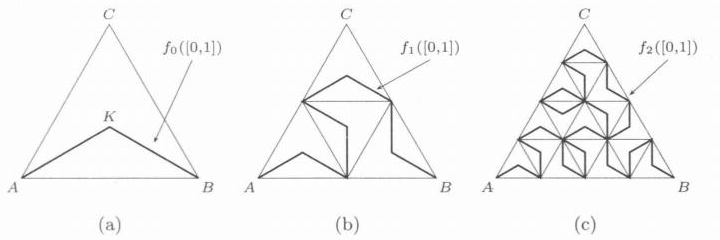
\includegraphics[width=.78\linewidth]{figures/lower/ch18/fig-18-1.png}

    图 18.1
  \end{center}

  \begin{enumerate}[label=(\arabic*)]
    \item 证明：任取 $n>m$，有
    \[
      \abs{f_n(t)-f_m(t)}\le\frac1{2^m},
    \]
    从而 $f_n(t)$（$n=1,2,\ldots$）在 $[0,1]$ 上一致收敛。设其极限映射为 $f$，证明 $f\colon[0,1]\to\Delta$ 连续；
    \item 证明：$f([0,1])=\Delta$，即连续映射 $f$ 把一个区间 $[0,1]$ 映为 $\RR^2$ 中的一个面积为 $\dfrac{\sqrt3}{4}$ 的区域 $\Delta$。
  \end{enumerate}
\end{xreferenceproblem}
\begin{xsolution}
固定 $m$。按构造，$f_m(t)$ 所在的第 $m$ 级小正三角形边长为 $2^{-m}$；之后每一步变换都保持该参数点的像留在这个第 $m$ 级小三角形中。因此对任意 $n>m$，$f_n(t)$ 与 $f_m(t)$ 位于同一个边长为 $2^{-m}$ 的小正三角形中。该三角形的直径就是边长，所以
\[
  \abs{f_n(t)-f_m(t)}\le\frac1{2^m},
  \qquad0\le t\le1.
\]
于是
\[
  \sup_{t\in[0,1]}\abs{f_n(t)-f_m(t)}
  \le\frac1{2^m},
  \qquad n>m.
\]
故 $\{f_n\}$ 是一致 Cauchy 列。$\RR^2$ 完备，所以存在映射 $f$ 使 $f_n\to f$ 在 $[0,1]$ 上一致。

每个 $f_n$ 都是有限条线段拼成的连续折线映射，连续函数列的一致极限连续，因此
\[
  \boxed{f\colon[0,1]\to\Delta\text{ 连续}}.
\]
令 $n\to\infty$ 于前面的估计，还得到
\[
  \sup_{t\in[0,1]}\abs{f(t)-f_m(t)}
  \le\frac1{2^m}.
\]
\end{xsolution}


\begin{xreferenceproblem}[8]
（Tietze（蒂策）扩张定理）设 $D\subset\RR^n$ 为闭子集，$f\colon D\to\RR$ 为连续函数，且
  \[
    \abs{f(\vect{x})}\le M,\qquad \vect{x}\in D.
  \]
  设 $g_0(\vect{x})=0$，$g_k(\vect{x})$ 归纳定义为
  \[
    g_k(\vect{x})=
    \frac{2^{k-1}d(\vect{x},A_k)}{3^k(d(\vect{x},A_k)+d(\vect{x},B_k))}
    -\frac{2^{k-1}d(\vect{x},B_k)}{3^k(d(\vect{x},A_k)+d(\vect{x},B_k))},
  \]
  其中
  \[
    A_k=\left\{\vect{x}\in D\mid\varphi_k(\vect{x})\ge\frac{2^{k-1}}{3^k}M\right\},
    \qquad
    B_k=\left\{\vect{x}\in D\mid\varphi_k(\vect{x})\le-\frac{2^{k-1}}{3^k}M\right\},
  \]
  而
  \[
    \varphi_k(\vect{x})
    =f(\vect{x})-[g_0(\vect{x})+g_1(\vect{x})+\cdots+g_{k-1}(\vect{x})],
    \qquad k=1,2,\ldots.
  \]
  \begin{enumerate}[label=(\arabic*)]
    \item 证明：$g_k(\vect{x})$（$k=1,2,\ldots$）连续，级数 $\displaystyle\sum_{k=1}^{\infty}g_k(\vect{x})$ 在 $\RR^n$ 上一致收敛到 $\RR^n$ 上的连续函数 $g(\vect{x})$，并且当 $\vect{x}\in D$ 时 $g(\vect{x})=f(\vect{x})$。因此 $g$ 称为 $f$ 在 $\RR^n$ 上的连续扩张，也称连续开拓；
    \item 证明：(1) 的结论当 $f$ 并不有界时也成立。
  \end{enumerate}
  （以上两题取自 [2]，又见 [3] 之 §16.3。）
\end{xreferenceproblem}
\begin{xsolution}
由每个 $f_m([0,1])\subset\Delta$ 且闭三角形 $\Delta$ 为闭集，一致极限逐点仍落在 $\Delta$ 中，因此 $f([0,1])\subset\Delta$。下面证明反向包含。

任取 $p\in\Delta$。第 $m$ 次等分把 $\Delta$ 分成边长为 $2^{-m}$ 的小正三角形。取其中一个包含 $p$ 的小三角形，记为 $\Delta_m(p)$。按构造，折线 $f_m([0,1])$ 在每个第 $m$ 级小三角形中都有一段，因此可取 $t_m\in[0,1]$，使
\[
  f_m(t_m)\in\Delta_m(p).
\]
同一小三角形内两点距离不超过其直径 $2^{-m}$，故
\[
  \abs{f_m(t_m)-p}\le\frac1{2^m}.
\]
由 (1) 的一致估计，
\[
  \abs{f(t_m)-f_m(t_m)}\le\frac1{2^m}.
\]
所以
\[
  \abs{f(t_m)-p}\le\frac2{2^m}\to0.
\]

区间 $[0,1]$ 紧，故 $\{t_m\}$ 有收敛子列
\[
  t_{m_j}\to t_*\in[0,1].
\]
由 $f$ 连续，
\[
  f(t_{m_j})\to f(t_*).
\]
另一方面，前面的估计给出 $f(t_{m_j})\to p$，故
\[
  f(t_*)=p.
\]
因此任意 $p\in\Delta$ 都属于 $f([0,1])$，从而
\[
  \boxed{f([0,1])=\Delta}.
\]
正三角形边长为 $1$，故面积为 $\sqrt3/4$。

题面所列递推式需要两处校正。若按题面原式，
\[
  \abs{g_k(\vect{x})}\le\frac{2^{k-1}}{3^k},
\]
故若原式处处有定义，则
\[
  \sum_{k=1}^\infty\abs{g_k(\vect{x})}
  \le\sum_{k=1}^\infty\frac{2^{k-1}}{3^k}=1.
\]
因此当 $M>1$ 且 $f$ 在某点取值大于 $1$ 时，原式不可能满足 $\sum g_k=f$。此外，若 $\vect{x}\in A_k$，原题所写公式给出的校正方向与减小正残差所需方向相反。

与 $A_k,B_k$ 的定义相容的递推式应为
\[
  \widetilde g_k(\vect{x})
  =a_kM\,
  \frac{d(\vect{x},B_k)-d(\vect{x},A_k)}
  {d(\vect{x},A_k)+d(\vect{x},B_k)},
  \qquad
  a_k=\frac{2^{k-1}}{3^k},
\]
当 $A_k,B_k$ 都非空时使用此式；若 $A_k=\varnothing,B_k\ne\varnothing$，取 $\widetilde g_k\equiv-a_kM$；若 $B_k=\varnothing,A_k\ne\varnothing$，取 $\widetilde g_k\equiv a_kM$；若二者皆空，取 $\widetilde g_k\equiv0$。以下证明这个修正式确实给出题目所要的结论。

令
\[
  \varphi_1=f,
  \qquad
  \varphi_k
  =f-\sum_{j=1}^{k-1}\widetilde g_j,
  \qquad k\ge2,
\]
在 $D$ 上定义。归纳证明
\[
  \abs{\varphi_k(\vect{x})}
  \le\left(\frac23\right)^{k-1}M
  =3a_kM,
  \qquad \vect{x}\in D.
\]
$k=1$ 时就是题设 $\abs{f}\le M$。

假设该估计对 $k$ 成立。由归纳假设，$\widetilde g_1,\ldots,\widetilde g_{k-1}$ 连续，故 $\varphi_k=f-\sum_{j=1}^{k-1}\widetilde g_j$ 在 $D$ 上连续。于是 $A_k,B_k$ 是 $D$ 中的闭集；又因 $D$ 本身闭，它们也是 $\RR^n$ 中的闭集。两集合由正、负阈值的定义互不相交。若二者非空，则距离函数连续且分母处处为正，所以 $\widetilde g_k$ 连续，并且
\[
  \abs{\widetilde g_k(\vect{x})}\le a_kM.
\]
在 $D$ 上分三种情况。

若 $\varphi_k(\vect{x})\ge a_kM$，则 $\vect{x}\in A_k$，因而
\[
  \widetilde g_k(\vect{x})=a_kM.
\]
结合 $\varphi_k\le3a_kM$ 得
\[
  0\le\varphi_{k+1}(\vect{x})
  =\varphi_k(\vect{x})-a_kM
  \le2a_kM.
\]
若 $\varphi_k(\vect{x})\le-a_kM$，则
\[
  \widetilde g_k(\vect{x})=-a_kM,
\]
从而
\[
  -2a_kM\le\varphi_{k+1}(\vect{x})\le0.
\]
若
\[
  \abs{\varphi_k(\vect{x})}<a_kM,
\]
则仅用 $\abs{\widetilde g_k}\le a_kM$ 即得
\[
  \abs{\varphi_{k+1}(\vect{x})}\le2a_kM.
\]
空集情形采用上面的常值约定时，同样得到这个估计。因此
\[
  \abs{\varphi_{k+1}(\vect{x})}
  \le2a_kM
  =\left(\frac23\right)^kM.
\]
归纳完成。

又因为
\[
  \sup_{\vect{x}\in\RR^n}
  \abs{\widetilde g_k(\vect{x})}
  \le a_kM,
\]
且
\[
  \sum_{k=1}^\infty a_kM=M<\infty,
\]
由 Weierstrass 判别法，级数
\[
  \sum_{k=1}^\infty\widetilde g_k(\vect{x})
\]
在 $\RR^n$ 上一致收敛。每一项连续，所以其和
\[
  g(\vect{x})=\sum_{k=1}^\infty\widetilde g_k(\vect{x})
\]
连续。

对 $\vect{x}\in D$，由残差估计
\[
  \abs*{f(\vect{x})-
  \sum_{j=1}^{k-1}\widetilde g_j(\vect{x})}
  =\abs{\varphi_k(\vect{x})}
  \le\left(\frac23\right)^{k-1}M\to0.
\]
故
\[
  g(\vect{x})=f(\vect{x}),
  \qquad\vect{x}\in D.
\]
这证明了修正递推式下的有界 Tietze 扩张结论。
\end{xsolution}


\begin{xreferenceproblem}[9]
是否能把开集上的连续函数连续扩张到全空间？一致连续函数呢？考察 $\RR$ 中的例子。
\end{xreferenceproblem}
\begin{xsolution}
使用 (1) 中已经得到的有界 Tietze 扩张结论。设 $f\colon D\to\RR$ 连续，但不要求有界。定义
\[
  h(\vect{x})
  =\frac{f(\vect{x})}{1+\abs{f(\vect{x})}},
  \qquad\vect{x}\in D.
\]
则 $h$ 连续且 $\abs{h(\vect{x})}<1$。由有界情形，存在连续函数
\[
  H\colon\RR^n\to[-1,1]
\]
使 $H|_D=h$。

令
\[
  Z=\{\vect{x}\in\RR^n\mid\abs{H(\vect{x})}=1\}.
\]
$Z$ 是闭集，且因 $\abs{h}<1$，有 $D\cap Z=\varnothing$。若 $Z=\varnothing$，令 $\lambda\equiv1$；若 $Z\ne\varnothing$，定义
\[
  \lambda(\vect{x})
  =\frac{d(\vect{x},Z)}
  {d(\vect{x},Z)+d(\vect{x},D)}.
\]
两个距离函数连续。由于 $D,Z$ 闭且不交，分母处处为正，所以 $\lambda$ 连续，并且
\[
  0\le\lambda\le1,
  \qquad
  \lambda|_D=1,
  \qquad
  \lambda|_Z=0.
\]
令
\[
  K(\vect{x})=\lambda(\vect{x})H(\vect{x}).
\]
则 $K$ 连续，$K|_D=h$，并且对每个 $\vect{x}\in\RR^n$ 都有 $\abs{K(\vect{x})}<1$：若 $\vect{x}\in Z$，则 $K(\vect{x})=0$；若 $\vect{x}\notin Z$，则 $\abs{H}<1$ 且 $0\le\lambda\le1$。

最后定义
\[
  G(\vect{x})
  =\frac{K(\vect{x})}{1-\abs{K(\vect{x})}}.
\]
因为 $\abs{K}<1$，$G$ 在全空间连续。对 $\vect{x}\in D$，$K=h$，而函数
\[
  u\longmapsto\frac{u}{1-\abs{u}}
\]
是 $t\mapsto t/(1+\abs{t})$ 在 $(-1,1)$ 上的反函数，所以
\[
  G(\vect{x})=f(\vect{x}).
\]
因此无界连续函数同样可以从闭集 $D$ 连续扩张到 $\RR^n$。

一般连续函数不能。取
\[
  U=(0,1)\subset\RR,
  \qquad
  f(x)=\frac1x.
\]
$f$ 在 $U$ 上连续。若存在连续扩张 $F\colon\RR\to\RR$，则由 $x\to0^+$ 应有
\[
  F(x)=\frac1x\to F(0)\in\RR,
\]
但 $1/x\to+\infty$，矛盾。因此开集上的连续函数未必能连续扩张到全空间。

若 $f$ 在开集 $U\subset\RR$ 上一致连续，则可以。先把它惟一连续扩张到闭包 $\overline U$。任取 $x\in\overline U$，取 $x_n\in U$、$x_n\to x$。由于 $f$ 一致连续，$\{f(x_n)\}$ 是 Cauchy 列，故收敛；一致连续性还保证其极限与所选逼近列无关。定义
\[
  \widetilde f(x)=\lim_{n\to\infty}f(x_n).
\]
同一个 $\varepsilon$--$\delta$ 条件传到极限后表明 $\widetilde f$ 在 $\overline U$ 上连续，并且 $\widetilde f|_U=f$。

现在 $\RR\setminus\overline U$ 是若干互不相交开区间的并。在每个有限空隙 $(a,b)$ 上，用连接 $\widetilde f(a)$ 与 $\widetilde f(b)$ 的线性函数定义扩张；在无界空隙 $(-\infty,a)$ 或 $(a,+\infty)$ 上取相邻端点值的常值函数。每个空隙内部的连续性直接成立，在空隙端点处也与 $\widetilde f$ 的端点值吻合。若有若干空隙的端点向 $x_0\in\overline U$ 聚集，则 $\widetilde f$ 在 $\overline U$ 上仍一致连续；足够靠近 $x_0$ 的空隙两端函数值都靠近 $\widetilde f(x_0)$，而线性插值位于两端函数值之间，故这些空隙内部的值也靠近 $\widetilde f(x_0)$。因此所得函数在全 $\RR$ 上连续，并在 $U$ 上与 $f$ 一致。

\textbf{另解（一致连续情形）。} 仍先由一致连续性把 $f$ 惟一连续扩张到闭集 $\overline U$。由于 $\overline U\subset\RR$ 是闭集，再应用上一题的 Tietze 扩张定理，即可把 $\widetilde f$ 连续扩张到整个 $\RR$。这直接得到所需的全空间连续扩张。

所以在 $\RR$ 中：一般连续函数的答案是否定的；一致连续函数的答案是肯定的。
\end{xsolution}


\begin{xreferenceproblem}[10]
证明：可以把定义在 $\RR^n$ 中有理点集上的一致连续函数惟一扩张到全空间。
\end{xreferenceproblem}
\begin{xsolution}
设有理点集为
\[
  D=\QQ^n\subset\RR^n,
\]
且 $f\colon D\to\RR$ 一致连续。任取 $\vect{x}\in\RR^n$，选有理点列
\[
  \vect{q}_m\in\QQ^n,
  \qquad
  \vect{q}_m\to\vect{x}.
\]
因为 $\{\vect{q}_m\}$ 是 Cauchy 列，而 $f$ 一致连续，所以 $\{f(\vect{q}_m)\}$ 也是 Cauchy 列，在 $\RR$ 中收敛。定义
\[
  F(\vect{x})=\lim_{m\to\infty}f(\vect{q}_m).
\]

先证定义与逼近列无关。若另有
\[
  \vect{r}_m\in\QQ^n,
  \qquad
  \vect{r}_m\to\vect{x},
\]
则
\[
  \abs{\vect{q}_m-\vect{r}_m}\to0.
\]
给定 $\varepsilon>0$，由一致连续性存在 $\delta>0$，使
\[
  \abs{\vect{u}-\vect{v}}<\delta
  \Longrightarrow
  \abs{f(\vect{u})-f(\vect{v})}<\varepsilon
\]
对所有有理点 $\vect{u},\vect{v}$ 成立。令 $m$ 足够大，得到
\[
  \abs{f(\vect{q}_m)-f(\vect{r}_m)}<\varepsilon,
\]
故两列极限相同。

若 $\vect{x}\in\QQ^n$，可取常值列 $\vect{q}_m=\vect{x}$，于是
\[
  F(\vect{x})=f(\vect{x}),
\]
故 $F$ 是扩张。

再证连续性，事实上 $F$ 仍一致连续。给定 $\varepsilon>0$，由原函数的一致连续性取 $\delta>0$，使对任意有理点 $\vect{u},\vect{v}$，
\[
  \abs{\vect{u}-\vect{v}}<\delta
  \Longrightarrow
  \abs{f(\vect{u})-f(\vect{v})}<\frac\varepsilon2.
\]
若
\[
  \abs{\vect{x}-\vect{y}}<\frac\delta3,
\]
分别选有理点列 $\vect{q}_m\to\vect{x}$、$\vect{r}_m\to\vect{y}$。当 $m$ 足够大时
\[
  \abs{\vect{q}_m-\vect{r}_m}<\delta,
\]
故
\[
  \abs{f(\vect{q}_m)-f(\vect{r}_m)}<\frac\varepsilon2.
\]
令 $m\to\infty$ 得
\[
  \abs{F(\vect{x})-F(\vect{y})}\le\frac\varepsilon2<\varepsilon.
\]
所以 $F$ 一致连续。

最后证惟一性。若 $G$ 是另一连续扩张，则对任意 $\vect{x}\in\RR^n$，取有理点列 $\vect{q}_m\to\vect{x}$，有
\[
  G(\vect{x})
  =\lim_{m\to\infty}G(\vect{q}_m)
  =\lim_{m\to\infty}f(\vect{q}_m)
  =F(\vect{x}).
\]
故 $G=F$，扩张惟一。
\end{xsolution}

